\documentclass[11pt]{article}
\usepackage{amsmath}
\usepackage{graphicx}
\usepackage{hyperref}
\usepackage[utf8]{inputenc}
\usepackage[spanish]{babel}
\usepackage[margin=2cm]{geometry}
\usepackage{amsfonts}
\usepackage{float}
\usepackage[procnames]{listings}
\usepackage{textcomp}
\usepackage{color}
\usepackage{hyperref}
\usepackage{rotating,booktabs}
\usepackage{subfigure}
\usepackage{caption}
\usepackage[T1]{fontenc}

% Custom colors
\definecolor{keywords}{RGB}{255,0,90}
\definecolor{comments}{RGB}{0,0,113}
\definecolor{red}{RGB}{160,0,0}
\definecolor{black}{RGB}{0,0,0}
 
\lstdefinestyle{python_style}{
    language=Python,
    frame=single,
    xleftmargin=.25in,
    upquote = true,
    basicstyle=\scriptsize,
    breakatwhitespace=false,         
    breaklines=true,                 
    captionpos=b,                    
    keepspaces=true,                 
    numbers=left,                    
    numbersep=5pt,                  
    showspaces=false,                
    showstringspaces=false,
    showtabs=false,                  
    tabsize=2,
    keywordstyle=\color{keywords},
    commentstyle=\color{comments},
    stringstyle=\color{red},
    identifierstyle=\color{black},
    procnamekeys={def,class}
}
 
\lstset{style=python_style}

\setlength{\belowdisplayskip}{5pt} 
\setlength{\belowdisplayshortskip}{5pt}
\setlength{\abovedisplayskip}{5pt} 
\setlength{\abovedisplayshortskip}{5pt}



\title{Clasificación de opiniones en tuits en español. Grupo: Equipo B.}
\author{David López Pretel - \href{mailto:derwey@correo.ugr.es}{derwey@correo.ugr.es} \\
Rshad Zhran - \href{mailto:rshadzhran@correo.ugr.es}{rshadzhran@correo.ugr.es} \\
Míriam Mengíbar Rodríguez - \href{mailto:mirismr@correo.ugr.es}{mirismr@correo.ugr.es} \\
Néstor Rodríguez Vico - \href{mailto:nrv23@correo.ugr.es}{nrv23@correo.ugr.es}}
\date{\today}

\begin{document}
\maketitle

\clearpage

\tableofcontents

\clearpage


\section{Introducción.}

En la actualidad, el auge de las redes sociales y su uso continuado provocan una cantidad enorme de datos de los que podemos sacar información muy valiosa. Es por ello que la minería de medios sociales es una rama de la ciencia de datos que trata de hacer esto. \\

En concreto, este trabajo trata de clasificar un \textit{tuit} en base a la opinión que el autor expresa, pudiendo clasificar un \textit{tuit} en alguna de las siguientes clases:

\begin{itemize}
    \item \textit{N}: \textit{tuit} con opinión negativa. En nuestro conjunto de entrenamiento hay 418 \textit{tuits} asociados a esta clase.
    \item \textit{P}: \textit{tuit} con opinión positiva. En nuestro conjunto de entrenamiento hay 318 \textit{tuits} asociados a esta clase.
    \item \textit{NEU}: \textit{tuit} con opinión neutra. En nuestro conjunto de entrenamiento hay 133 \textit{tuits} asociados a esta clase.
    \item \textit{NONE}: \textit{tuit} sin opinión. En nuestro conjunto de entrenamiento hay 139 \textit{tuits} asociados a esta clase.
\end{itemize}

Para esta tarea de clasificación hemos hecho uso de redes neuronales usando la librería \textit{keras} y \textit{tensorflow}. Además, se detallará el preprocesamiento realizado a los \textit{tuits}, las distintas arquitecturas, los experimentos realizados y, por último, los resultados obtenidos.

\section{Metodología de trabajo.}

Para la elección de los modelos en la competición, se ha usado la estrategia \textit{K-Fold Cross Validation} con \textit{K=5}. En nuestro caso, hemos unido el conjunto de \textit{train} y \textit{validation} y, sobre este nuevo conjunto, hemos realizado las distintas particiones. \\

Para cada modelo usado, se ha pintado una gráfica donde se muestra el como evoluciona el valor de la función \textit{loss} en el conjunto de entrenamiento y el conjunto de validación para cada partición del \textit{K-Fold Cross Validation} a lo largo de las épocas de aprendizaje. También, se ha pintado la media de todas las particiones. \\

A la hora de comparar las clases predichas con las clases reales se ha usado la métrica \textit{F1 score}, la cual se define como:

\begin{equation}
    2 * \frac{precision \cdot recall}{precision + recall}
\end{equation}

Dicha métrica se ha calculado en dos versiones:

\begin{itemize}
    \item \textit{micro}: Calcula las métricas globalmente contando el total de los verdaderos positivos, falsos negativos y falsos positivos.
    \item \textit{macro}: Calcula las métricas para cada etiqueta y encuentre su media no ponderada. Esta no tiene en cuenta el desequilibrio de la etiqueta.
\end{itemize}

Al igual que se ha hecho con la gráfica de la función \textit{loss}, se ha calculado el valor de las métricas \textit{micro-f1} y \textit{macro-f1} para cada partición y se han usado como métricas finales del modelo la media de las mismas.

\section{Estudio y preparación de los datos.}

En esta sección se describe cómo se han leído los datos, el procesamiento realizado a los \textit{tuits} y cómo se ha balanceado el conjunto de datos mediante \textit{oversampling}.

\subsection{Lectura de datos.}

Para la lectura de datos se ha usado la función \textit{parse} de la biblioteca \textit{xml.etree.ElementTree}, la cual es estándar de \textit{Python}. A continuación, se han creado objetos de una clase \textit{Tweet} (creada por nosotros para la lectura de datos) para los conjuntos \textit{train} y \textit{validation}. A continuación se ha extraído el texto del \textit{tuit}, el identificador y la clase del mismo.

\subsection{Preprocesamiento.} \label{preprocesamiento}
El hecho de que los datos vengan de una fuente tan diversa como una red social, requiere un preprocesamiento exhaustivo y específico. Cada usuario expresará sus opiniones de formas muy diversas, por lo que en este apartado intentaremos ser capaces de transformar los datos de forma que los \textit{tuits} que pertenezcan a una misma clase sean lo más similares posible. Describamos una a una las distintas etapas que se han seguido para lograr este objetivo.
\\

En primer lugar, lo que haremos será convertir todo el texto de cada \textit{tuit} a minúscula y sin acentos. Es evidente pensar que esto hará que los textos de los diferentes \textit{tuits} se asemejen más sin cambiar su significado. Además, se eliminarán signos de puntuación, caracteres como \textit{\&} o \textit{\-} y aquellas letras que aparezcan repetidas más de dos veces. Por ejemplo, si tenemos la palabra \textit{hooootel} la transformaremos a \textit{hotel}. A continuación, para los \textit{hashtag}, eliminaremos el carácter \textit{\#} aunque si dejaremos el \textit{hashtag} en cuestión, pues este puede estar relacionado con algún tipo de opinión (p.e, el \#felicidad podría estar normalmente asociado a un \textit{tuit} positivo. Así mismo, eliminaremos la cadena \textit{rt} que no aporta nada de información al contenido. Por último, terminaremos esta primera etapa reduciendo espacios múltiples a un solo espacio.
\\

Como segunda etapa de preprocesamiento, haremos un tratamiento específico de los \textit{emojis}. Hemos agrupado los \textit{emojis} según la emoción que expresen. Una vez hecho esto, reemplazaremos el \textit{emoji} por \textit{POSITIVE} en caso de expresar una emoción positiva (p. e, \textit{$:)$ )} o por \textit{NEGATIVE} en caso de expresar una opinión negativa (p. e, \textit{$:($ )}. Así mismo, las risas se han reemplazado por \textit{POSITIVE}. Sobre esta idea, hemos aplicado un proceso simple para premiar a los \textit{tuits} que contenga \textit{emojis}: parece lógico pensar que si un \textit{tuit} tiene un \textit{emoji} es más probable que la clasificación de este \textit{tuit} sea a la emoción que expresa dicho \textit{emoji}. Es por ello, que cada uno de ellos será reemplazado por cuatro repeticiones de \textit{POSITIVE} o de \textit{NEGATIVE} según corresponda.
\\

En la tercera etapa, tratamos de hacer un procedimiento similar a la anterior pero, en este caso, con palabras malsonantes. Una palabra malsonante puede ser, por ejemplo, un insulto. Para ello, se ha construido una lista de forma manual de algunas palabras mal sonantes, ya que, en español, no hemos encontrado una lista completa de dichas palabras. Cada palabra malsonante será reemplazada por cuatro repeticiones de \textit{NEGATIVE}, debido a que parece lógico que este \textit{tuit} exprese un sentimiento negativo.
\\

Como cuarta etapa, se ha procedido a convertir todos los números (escritos numéricamente) a texto. Esto permite que si el texto de dos \textit{tuits} distintos fuesen \textit{``12''} y \textit{``doce''}, tengan el mismo contenido.
\\

Como etapa opcional, podemos indicar si queremos quedarnos con la raíz de cada palabra. Esto permite que, por ejemplo, conjugaciones del mismo verbo o palabras con la misma raíz sean lo mismo: \textit{gustar, gusto, gustaría...} Sin embargo, esto puede hacernos perder información al eliminar parte de las palabras.
\\

Por último, si analizamos las palabras más frecuentes de todos los \textit{tuits} mediante \textit{wordclouds} nos encontramos que palabras con apenas significado semántico, son las que más aparecen (el tamaño de la palabra es proporcional a la veces que aparece, es decir, cuánto más grande sea su tamaño, más veces aparecerá). Se muestran en las siguientes imágenes las \textit{wordclouds} para todos los \textit{tuits} de cada clase en los conjuntos de \textit{train} y \textit{validation}.

\begin{figure}[H]
\includegraphics[width=\linewidth]{images/wordcloud/wordcloud_train.png}
\caption{\textit{Wordcloud} del conjunto de \textit{train} para cada clase.}
\end{figure}

\begin{figure}[H]
\includegraphics[width=\linewidth]{images/wordcloud/wordcloud_validation.png}
\caption{\textit{Wordcloud} del conjunto de \textit{validation} para cada clase.}
\end{figure}

Vemos que en casi todas las clases se repiten las mismas palabras aproximadamente para los dos conjuntos de datos. Dichas palabras se las conoce como \textit{stopwords}. Este conjunto de palabras está formado por preposiciones, artículos, conjunciones, etc. Por tanto, en esta última etapa de preprocesamiento trataremos de eliminarlas. Para ver el efecto que esto supone, se vuelven a mostrar las \textit{wordclouds} de ambos conjuntos (\textit{train} y \textit{validation}) para las distintas clases.

\begin{figure}[H]
\includegraphics[width=\linewidth]{images/wordcloud/wordcloud_train_preprocessed.png}
\caption{\textit{Wordcloud} del conjunto de \textit{train} preprocesado para cada clase.}
\end{figure}

\begin{figure}[H]
\includegraphics[width=\linewidth]{images/wordcloud/wordcloud_validation_preprocessed.png}
\caption{\textit{Wordcloud} del conjunto de \textit{validation} preprocesado para cada clase.}
\end{figure}

Si observamos las \textit{wordclouds} preprocesadas, vemos como en la clase positiva la palabra \textit{POSITIVE} se repite bastante, lo cual puede indicar que nuestras suposiciones a la hora de reemplazar los \textit{emojis} es buena. Así mismo, vemos palabras como \textit{gracias, genial, bien} y \textit{bueno} entran en las positivas y palabras como \textit{triste, dinero, malo} y \textit{llorar} aparecen en las negativas. Sin embargo, vemos que para la clase \textit{NONE} no hay ninguna palabra que identifique sentimientos positivos o negativos. En la clase \textit{NEU}, se mezclan bastantes palabras sin nada que destacar aparentemente.

\subsection{Oversampling.}
Dado que hay una clara desigualdad entre las clases de los datos (hay 318 elementos de la clase \textit{P}, hay 418  elementos de la clase \textit{N}, hay 139 elementos de la clase \textit{NONE} y 133 elementos de la clase \textit{NEU}) creemos que aplicar técnicas que afronten los problemas de clasificación no balanceada puede aportar buenos resultados. Para ello se ha elegido el método de \textit{oversampling} \textit{SMOTE}. Dicho método se encarga de crear muestras sintéticas interpolando las muestras de la clase minoritaria con un vecino aleatorio de sus $k$ vecinos más cercanos.\\

Para aplicar \textit{SMOTE} a los datos de los que disponemos ha sido necesario crear una \textit{bolsa de palabras} ya que será la representación en forma de vector que permita al algoritmo interpolar nuevas instancias y, por tanto, nuevos \textit{tuits}. Para la creación de la bolsa de palabras se ha creado un vocabulario que contiene todos los token pertenecientes a todos los \textit{tuits} y a partir de ese vocabulario se ha representado cada \textit{tuit} en forma de vector de 0's y 1's, añadiendo un 1 en el índice correspondiente a la palabra del vocabulario. Una vez obtenida la representación basta con aplicar \textit{SMOTE} y revertir el proceso, es decir, pasar de la \textit{bolsa de palabras} a los \textit{tuits}. A la hora de crear el vocabulario se han obviado las comas, puntos y demás caracteres especiales ya que se generarían \textit{tuits} sintéticos con dichos caracteres en posiciones no comunes y tampoco marcan una diferencia a la hora de clasificar la etiqueta.

\begin{figure}[H]
\centering
\includegraphics[scale=0.5]{images/bag_of_words.png}
\caption{Ejemplo de bolsa de palabras}
\end{figure}

\section{Modelos de redes.} \label{models}

En esta sección se describirán las partes comunes a los distintos modelos y modelos de redes que se han probado. Para ello, se mostrará el código \textit{Python} junto a una breve explicación de los razonamientos seguidos para su construcción. \\

Todas las redes mostradas a continuación tienen los siguientes puntos en común:

\begin{itemize}
    \item Reciben como entrada el conjunto de entrenamiento junto con sus etiquetadas y el conjunto de test con sus etiquetas. En el proceso de elección del modelo, el conjunto de test será el conjunto \textit{validation}, del cual disponemos de las etiquetas y pueden ser pasadas al modelo. Estás etiquetas son las usadas para validar el modelo internamente durante el proceso de aprendizaje y, de esta manera, poder pintar la gráfica comentada anteriormente. En la fase de predicción, el conjunto de test que recibe la red es el conjunto de test disponible, del cual no disponemos las etiquetadas y por lo tanto no se generará la gráfica para dicha ejecución.
    \item Un argumento \textit{verbose}, para indicar si se puedas información del proceso de aprendizaje o no.
    \item Los argumentos necesarios para la propia red, como puede ser el número de épocas o el valor de \textit{learning rate} deseado.
    \item Lo primero que haces es llamar a la función \textit{own\_set\_seed()} para ``setear'' las semillas de todos las librerías usadas para poder reproducir los resultados.
\end{itemize}

A parte de lo comentado anteriormente, hay una serie de funciones y variables declaradas y usadas por las redes:

\begin{itemize}
    \item \textit{\_\_CLASSES\_\_}: Variable usada para almacenar las clases disponibles.
    \item \textit{\_\_CLASSES\_TO\_NUM\_DIC\_\_}: Diccionario usado para mapear cada clase a un valor numérico.
    \item \textit{\_\_NUM\_TO\_CLASSES\_DIC\_\_}: Diccionario usado para mapear un valor numérico a cada clase.
    \item \textit{tokenize}: función usada para tokenizar un \textit{tuit}.
    \item \textit{fit\_transform\_vocabulary}: Función para crear el vocabulario a partir del \textit{corpus} de entrenamiento.
    \item \textit{fit\_transform\_vocabulary\_pretrain\_embeddings}: Función para crear el vocabulario a partir del \textit{corpus} de entrenamiento y un conjunto preentrenado de \textit{embeddings}.
    \item \textit{read\_embeddings}: Función para leer un fichero de \textit{embeddings}.
\end{itemize}

\subsection{tfidf\_rnn.} \label{tfidfrnn}

La primera red que hemos probado es una red básica que aplica el algoritmos \textit{tfidf}. Esta red no usa \textit{embeddings}, sino el concepto \textit{frecuencia de término - frecuencia inversa de documento}. Esa idea es una medida numérica que expresa cómo de relevante es una palabra para un documento en una colección. El proceso de montar la información necesaria para \textit{tfidf} lo podemos ver en las líneas \textit{15-29}. La arquitectura usada en esta red es una arquitectura estándar: 

\begin{itemize}
    \item Capa de entrada \textit{LSTM} con 64 neuronas.
    \item Capa oculta \textit{Dense} con 32 neuronas y \textit{tanh} como función de activación.
    \item Capa oculta \textit{Flatten}, para ``aplanar'' la salida.
    \item Capa de salida \textit{Dense} con \textit{numero de clases} neuronas y \textit{softmax} como función de activación, para poder obtener una distribución de probabilidad que nos permita decidir a que clase pertenece la entrada.
\end{itemize}

Una vez tenemos la información necesaria para \textit{tfidf} y la red definida, convertimos la entrada a sus ``valores'' \textit{tfidf} correspondientes (líneas \textit{45-55}) y entrenamos la red (líneas \textit{58-63}), para predecir la salida en la línea \textit{65}.

\lstinputlisting{src/tfidf_rnn.py}

\subsection{calculated\_embeddings\_rnn.} \label{calculatedembeddingsrnn}

Esta es la primera red en la que vamos a usar el concepto de \textit{Embedding}. Un \textit{embedding} es la representación de una palabra o frase del vocabulario en forma de un vector de número reales. Conceptualmente, nos permite representar las palabras en un espacio \textit{N}-dimensional sobre el cual podemos aplicar operaciones de vectores para determinar las relaciones entre las palabras de nuestro vocabulario. En este caso, vamos a calcular los \textit{embeddings} asociados a nuestro conjunto de entrenamiento en la propia red (líneas \textit{14-24}). Una vez tenemos los \textit{embeddings} montamos una red con la siguiente arquitectura:
\begin{itemize}
    \item Capa \textit{Embedding} como capa de entrada.
    \item Capa oculta \textit{LSTM} con 64 neuronas.
    \item Capa oculta \textit{Dense} con 32 neuronas y \textit{tanh} como función de activación.
    \item Capa oculta \textit{Flatten}, para ``aplanar'' la salida.
    \item Capa de salida \textit{Dense} con \textit{numero de clases} neuronas y \textit{softmax} como función de activación, para poder obtener una distribución de probabilidad que nos permita decidir a que clase pertenece la entrada.
\end{itemize}

Una vez tenemos los \textit{embeddings} y la red definida, mapeamos la entrada a sus \textit{embeddings} correspondientes (líneas \textit{37-42}) y entrenamos la red (líneas \textit{44-49}), para predecir la salida en la línea \textit{51}.
\lstinputlisting{src/calculated_embeddings_rnn.py}

\subsection{pretrain\_embeddings\_rnn.} \label{pretrainembeddingsrnn}

Una vez hemos introducido el concepto de \textit{embedding}, podemos ir un paso más allá. Construir un conjunto de \textit{embeddings} usando sólo las palabras disponibles en nuestro conjunto de entrenamiento puede llevarnos a generar unos \textit{embeddings} que no sean de calidad y que no representen realmente lo que queremos que representen. Por lo tanto, surgen técnicas e ideas de generar un conjunto de \textit{embeddings} a partir de un conjunto de entrenamiento lo suficientemente grande y descriptivo del lenguaje empleado en el problema a resolver. Esta red hace uso de un fichero de \textit{embeddings} ya existente, el cual se específica en el argumento \textit{embeddings\_path}. A parte de los \textit{embeddings} definimos dos nuevas entradas para poder lidiar con palabras que no están en el conjunto de \textit{embeddings} y otra para rellenar la entrada de la red si esta no es lo suficientemente grande como para cubrir todas las neuronas de entrada. Con estos \textit{embeddings} montamos nuestro vocabulario de entrenamiento (líneas \textit{17-22}). A continuación montamos una red con la siguiente arquitectura:

\begin{itemize}
    \item Capa \textit{Embedding} como capa de entrada.
    \item Capa oculta \textit{LSTM} con 64 neuronas.
    \item Capa oculta \textit{Dense} con 32 neuronas y \textit{tanh} como función de activación.
    \item Capa oculta \textit{Flatten}, para ``aplanar'' la salida.
    \item Capa de salida \textit{Dense} con \textit{numero de clases} neuronas y \textit{softmax} como función de activación, para poder obtener una distribución de probabilidad que nos permita decidir a que clase pertenece la entrada.
\end{itemize}

Finalmente, mapeamos la entrada a sus \textit{embeddings} correspondientes (líneas \textit{51-55}) y entrenamos la red (líneas \textit{58-62}), para predecir la salida en la línea \textit{64}.

\lstinputlisting{src/pretrain_embeddings_rnn.py}

\subsection{sigmoid\_pretrain\_embeddings\_rnn.} \label{sigmoidpretrainembeddingsrnn}

Una vez tenemos claro que lo mejor es usar un conjunto de \textit{embeddings} obtenido sobre un conjunto de entrenamiento grande, veamos que más podemos hacer en una red. Una de las cosas que hemos hecho hasta ahora es usar la función de tangente hiperbólica como la función de activación de la primera capa \textit{Dense} de nuestras redes. Dicha función tiene la siguiente forma:

\begin{figure}[H]
\centering
\includegraphics[width=0.5\linewidth]{images/tanh.png}
\end{figure}

Sin embargo, otra de las funciones clásicas para Redes Neuronales es la función \textit{sigmoide}, la cual tiene la siguiente forma:

\begin{figure}[H]
\centering
\includegraphics[width=0.5\linewidth]{images/sigmoid.png}
\end{figure}

Como podemos ver, la función \textit{tanh} es una función que toma valores de \textit{-1} a \textit{1} mientras que la función \textit{sigmoide} toma valores de \textit{0} a \textit{1}. En esta red hemos querido probar la función \textit{sigmoide} (línea \textit{40}) para ver cómo influye la función de activación elegida.

\lstinputlisting{src/sigmoid_pretrain_embeddings_rnn.py}

Tras los experimentos realizados, hemos visto que \textit{tanh} ofrece mejores resultados. Buscando información hemos aprendido que las \textit{LSTMs} tienen un vector interno para representar que pesos pueden crecer o decrecer en el proceso de aprendizaje. La función \textit{sigmoide} genera siempre valores positivos y, por lo tanto, los valores de los pesos sólo pueden crecer. Sin embargo, \textit{tanh} genera valores positivos y negativos, permitiendo así que los pesos crezcan y decrezcan, lo cual da más flexibilidad en el proceso de aprendizaje ya que da más libertad para que los pesos se ajusten.

\subsection{stacked\_lstm\_rnn.} \label{stackedlstmrnn}

Tal y como hemos estado viendo, lo mejor es trabajar con la función \textit{tanh} y \textit{embeddings} pre-entrenados. La siguiente prueba que hemos hecho es aumentar el número de capas de la red, para tener así una red más compleja. La idea detrás del uso de redes neuronales en \textit{Deep Learning} es precisamente, tener redes con varias capas ocultas que permitan un aprendizaje más detallado del problema. Por ello, la arquitectura usada para esta red es la siguiente:

\begin{itemize}
    \item Capa \textit{Embedding} como capa de entrada.
    \item Cuatro capas ocultas \textit{LSTM} con 64 neuronas cada una.
    \item Capa oculta \textit{Dense} con 32 neuronas y \textit{tanh} como función de activación.
    \item Capa oculta \textit{Flatten}, para ``aplanar'' la salida.
    \item Capa de salida \textit{Dense} con \textit{numero de clases} neuronas y \textit{softmax} como función de activación, para poder obtener una distribución de probabilidad que nos permita decidir a que clase pertenece la entrada.
\end{itemize}

\lstinputlisting{src/stacked_lstm_rnn.py}

En nuestro caso particular, aumentar el número de capas ocultas no ha mejorado los resultados obtenidos.

\subsection{adadelta\_rnn.} \label{adadeltarnn}

Otra de las cosas que podemos modificar de una red es el optimizador usada por la misma. En todos los ejemplos mostrados hasta ahora el optimizador usado ha sido \textit{adam} (\href{https://arxiv.org/abs/1412.6980v8}{Adam: A Method for Stochastic Optimization}). En \href{http://cs231n.github.io/neural-networks-3/#ada}{http://cs231n.github.io/neural-networks-3/\#ada} podemos ver un \textit{gif} que nos muestra cómo varía el comportamiento de una red en base al optimizador usado. Si nos quedamos con el momento inicial y el momento final del \textit{gif} tenemos lo siguiente:

\begin{table}[H]
\centering
\begin{tabular}{cc}
\includegraphics[width=0.4\linewidth]{images/optimizers_1.png} & \includegraphics[width=0.4\linewidth]{images/optimizers_2.png}
\end{tabular}
\end{table}

A pesar de que todos parten del mismo punto (figura de la izquierda), el camino recorrido para llegar a la solución, representada como una estrella, es totalmente distinto. Si observamos el \textit{gif}, también podremos apreciar la diferencia de velocidad para encontrar dicha solución. Si nos fijamos, el que mejores resultados da es \textit{adadelta}, y por lo tanto lo hemos probado. La red usada es la misma que la explicada en la sección \textit{pretrain\_embeddings\_rnn} (\ref{pretrainembeddingsrnn}) pero usando \textit{adadelta} (línea \textit{43}) como optimizador.

\lstinputlisting{src/adadelta_rnn.py}

\subsection{calculated\_embeddings\_LSTM\_CONV.} \label{calculatedembeddingsLSTMCONV}

Hasta ahora, nos hemos centrado en capas \textit{LSTM} pero queremos probar también cómo funcionan las capas convolucionales en procesamiento de texto. Para ello, hemos diseñado una red que combina ambas neuronas. La arquitectura usada para esta red es la siguiente:

\begin{itemize}
    \item Capa \textit{Embedding} como capa de entrada.
    \item Capa \textit{LSTM}, con 64 neuronas y con un \textit{Dropout} al 50\% de las neuronas.
    \item Capa oculta de \textit{pooling}, mediante la función \textit{Maxpooling1D}.
    \item Capa oculta de convolución con \textit{Conv1D}, con 128 neuronas,  y con un \textit{Dropout} al 50\% de las neuronas.
    \item Capa oculta de \textit{pooling} con la función \textit{AveragePooling1D()}.
    \item Capa oculta \textit{Dense} con 128 neuronas y \textit{relu} como función de activación.
    \item Capa oculta \textit{Flatten}, para ``aplanar'' la salida.
    \item Capa de salida \textit{Dense} con \textit{numero de clases} neuronas y \textit{softmax} como función de activación, para poder obtener una distribución de probabilidad que nos permita decidir a que clase pertenece la entrada.
\end{itemize}

La idea de usar un modelo que combine \textit{LSTM} y \textit{CNN} es que \textit{LSTM} permite almacenar información no solo del token actual, sino también de cualquier token anterior. La salida de la capa \textit{LSTM} se introduce en una capa de convolucional para extraer las características locales. \\

Más particularmente, si hablamos del uso de \textit{CNN} y dónde puede ayudar, en nuestro caso particular, podría capturar una frase negativa como ``no me gusta'', independientemente de dónde suceda en el \textit{tuit}, como por ejemplo:

\begin{itemize}
    \item No me gusta ver ese tipo de películas.
    \item Esa es la única cosa que realmente no me gusta.
    \item Vi la película, y no me gusta cómo terminó.
\end{itemize}

\begin{figure}[H]
\centering
\includegraphics[width=0.5\linewidth]{images/lstm-cnn-konukoii-1024x535.png}
\end{figure}

\lstinputlisting{src/calculated_embeddings_LSTM_CONV.py}

\subsection{pretrain\_embeddings\_LSTM\_CONV.}

Al igual que hemos propuesto usar \textit{embeddings} para redes \textit{LSTM}, hemos pensado que obtendríamos una mejora si usamos \textit{embeddings} pre-entrenados con esa nueva arquitectura de red.

\label{pretrainembeddingsLSTMCONV}
\lstinputlisting{src/pretrain_embeddings_LSTM_CONV.py}

\subsection{big\_LSTM\_CONV\_rnn.} \label{bigLSTMCONVrnn}

En este modelo, se ha seguido el concepto de \textit{stacked models}, en otras palabras, considerar un modelo de los explicados anteriormente como una capa. En este caso, hemos utilizado el modelo \textit{LSTM-CNN} varias veces en forma de pila. En los experimentos realizados, hemos podido observar que este modelo tiene un gran sobreaprendizaje. Este sobre aprendizaje se produce por la manera de aprendizaje que se implementa y la que se puede resumir como lo siguiente: Una capa \textit{LSTM} sirve para memorizar y capturar el cambio de sentimientos en un \textit{tuit}, dando más peso al sinónimo que refiere a un sentimiento pero que aparece al final del texto. Por ejemplo si tenemos el siguiente \textit{tuit}: \textit{Al principio me encantó, pero luego terminé odiándolo}. En este caso aparecen 2 sentimientos diferentes en la frase que son totalmente opuestos, pero claramente este \textit{tuit} nos dice que al final la persona acabó con odio y no con gusto. Y como ya hemos mencionado antes una capa \textit{CNN} ayuda a capturar la negatividad en un texto. Juntar varias capas para analizar el sentimiento que aparece en un texto que consideramos corto, no es oportuno, porqué aumentar el número de capas ocultas puede aumentar la precisión en clasificación pero hacer que el modelo aprendido sea demasiado específico. Analizar \textit{tuits} de unas 10 o 20 palabras no es una tarea \textit{compleja} y, por lo tanto, no necesitamos ese sobreajuste en el proceso de aprendizaje.

\lstinputlisting{src/big_LSTM_CONV_rnn.py}


\subsection{dropout\_LSTM\_CONV\_rnn.} \label{dropoutLSTMCONVrnn}

Este modelo es una versión modificada de \textit{pretrain\_embeddings\_LSTM\_CONV} en la que aumentamos el valor de \textit{Dropout} de 0.5 a 0.7, es decir, aplicamos la técnica de \textit{Dropout} al 70\% de las neuronas de la capa. La motivación de esta red ha sido intentar reducir el sobreabrendizaje. A nivel práctico, este modelo ha producido una mejora en la puntuación de \textit{Kaggle}, pasando de un \textit{0.51845} con \textit{dropout = 0.5} a un \textit{0.54305} \textit{dropout = 0.7}.

\lstinputlisting{src/dropout_LSTM_CONV_rnn.py}

\subsection{bidirectional\_lstm\_rnn.} \label{bidirectionallstmrnn}

Las neuronas \textit{LSTM} usadas hasta ahora son unidireccionales, esto quiere decir que, en su núcleo, preservan la información de las entradas que ya han pasado por dicha neurona. Es decir, las \textit{LSTM} unidireccionales sólo conservan información del pasado porque las únicas entradas que han visto son del pasado. Si usamos \textit{LSTM} bidireccionales, la entrada será pasada por la neurona de dos maneras, una primera vez de \textit{pasado al futuro} y otra del \textit{futuro al pasado}. Este enfoque permite conservar información del pasado y del futuro en dos estados dentro de la neurona. De esta manera, si los combinamos, somos capaces de, en cualquier momento, tener información tanto del pasado como del futuro. Veamos esto con un ejemplo. Supongamos que estamos en un problema de predicción de la siguiente palabra cuando estamos escribiendo, tal y como puede hacer el auto-corrector que usamos todos los días en los móviles. A muy alto nivel, una capa formada por neuronas \textit{LSTM} unidireccionales podría ver \textit{Ellos fueron...}. En ese momento, intentamos predecir la siguiente palabra. Si usamos una red con capas formadas por neuronas \textit{LSTM} bidireccionales podemos ver la información con más detalle, teniendo una información \textit{desde el pasado al futuro}, como podría ser \textit{Ellos fueron a comer...} e información \textit{desde el futuro al pasado}, como \textit{... y luego a jugar}. Si permitimos que la red aprenda el contexto en ambos sentidos. \\

La red usada es la misma que la explicada en la sección \textit{pretrain\_embeddings\_rnn} (\ref{pretrainembeddingsrnn}) pero con neuronas \textit{LSTM} bidireccionales tal y como podemos ver en la línea \textit{41}.

\lstinputlisting{src/bidirectional_lstm_rnn.py}

\subsection{pretrained\_embeddings\_cnn\_bidirectional\_LSTM.}

Al igual que hemos probado a combinar capas \textit{LSTM} con capas convolucionales, hemos combinado la versión bidireccional de estas últimas, teniendo así una red que mezcla neuronas convolucionales (línea \textit{47}) y neuronas de \textit{pooling} (línea \textit{49}), ambas características de redes \textit{CNN}, con neuronas \textit{LSTM} bidireccionales (línea \textit{54}).

\label{pretrainedembeddingscnnbidirectionalLSTM}
\lstinputlisting{src/pretrained_embeddings_cnn_bidirectional_LSTM.py} 

\section{Experimentos.}

En esta sección se describirán los distintos experimentos realizados, combinando las arquitecturas de las redes con distintos parámetros y métodos de preprocesamiento. Para cada experimento se va a mostrar la gráfica de la función \textit{loss} comentada anteriormente, un resumen de la arquitectura de la red obtenida con la función \textit{summary} de \textit{keras} aplicada sobre el modelo de red y el valor de \textit{macro\_f1}, \textit{micro\_f1} y el valor obtenido en la competición de \textit{kaggle}. \\

Cuando se muestre el resumen de la arquitectura, no se va a hacer en gran detalle porque se ha comentado en la sección \ref{models}. En esta sección comentaremos más el número de parámetros que tiene la red, ya que esto define la complejidad de la misma y el número de parámetros entrenables frente al número de parámetros no entrenables. Un parámetro entrenable es un parámetro cuyo valor varía durante el aprendizaje. En \textit{keras} podemos tener varios tipos de parámetros no entrenables:

\begin{itemize}
    \item Parámetros que han sido marcados como constantes. Esto significa que \textit{keras} no los actualizará durante el entrenamiento.
    \item Parámetros estadísticos en las capas \textit{BatchNormalization}. Estos se actualizan con la media y la varianza, pero no están con el proceso de \textit{backpropagation}.
    \item Parámetros de entrada de la propia red, como pueden ser los \textit{embeddings}.
\end{itemize}

De no indicarse lo contrario, los \textit{embeddings} usados en todas las redes han sido los proporcionados por el profesorado de asignatura en las clases de prácticas, es decir, \textit{fasttext\_spanish\_twitter\_100d.vec}.

\subsection{tfidf\_rnn.} \label{exp_tfidfrnn}

Experimento generado usando la red descrita en la sección \textit{tfidf\_rnn} (\ref{tfidfrnn}) usando los parámetros por defecto indicados en la misma.

\begin{figure}[H]
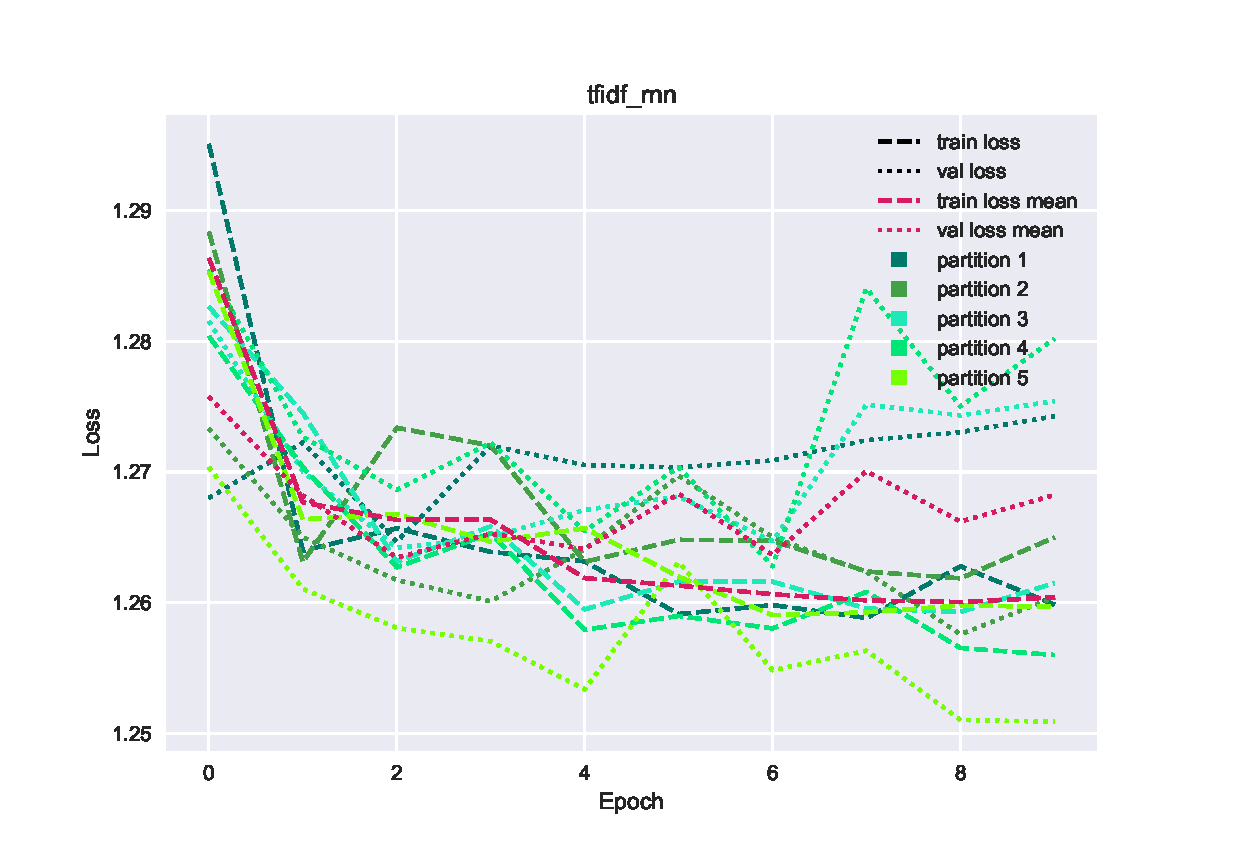
\includegraphics[width=\linewidth]{images/loss/tfidf_rnn-1554202898.eps}
\end{figure}

Como podemos ver, el valor de la función \textit{loss} decrece según van pasando las épocas, tanto para el conjunto de \textit{train} como para el conjunto de \textit{validation}. Esta es la situación que nos interesa ver en este tipo de gráficas. Veamos ahora la arquitectura de la red:

\begin{verbatim}
Layer (type)                 Output Shape              Param #   
=================================================================
lstm_1 (LSTM)                (None, 29, 64)            16896     
dense_1 (Dense)              (None, 29, 32)            2080      
flatten_1 (Flatten)          (None, 928)               0         
dense_2 (Dense)              (None, 4)                 3716      
=================================================================
Total params: 22,692
Trainable params: 22,692
Non-trainable params: 0
\end{verbatim}

Como podemos ver, todos los parámetros de la red son entrenables. Los resultados de este experimento son: 

\begin{table}[H]
\begin{tabular}{c|c|c}
\textbf{macro\_f1:} 0.159393 & \textbf{micro\_f1:} 0.414133 & \textbf{kaggle:} 0.42179
\end{tabular}
\end{table}

\subsection{calculated\_embeddings\_rnn.} \label{exp_calculatedembeddingsrnn}

Experimento generado usando la red descrita en la sección \textit{calculated\_embeddings\_rnn} (\ref{calculatedembeddingsrnn}) usando los parámetros por defecto indicados en la misma.

\begin{figure}[H]
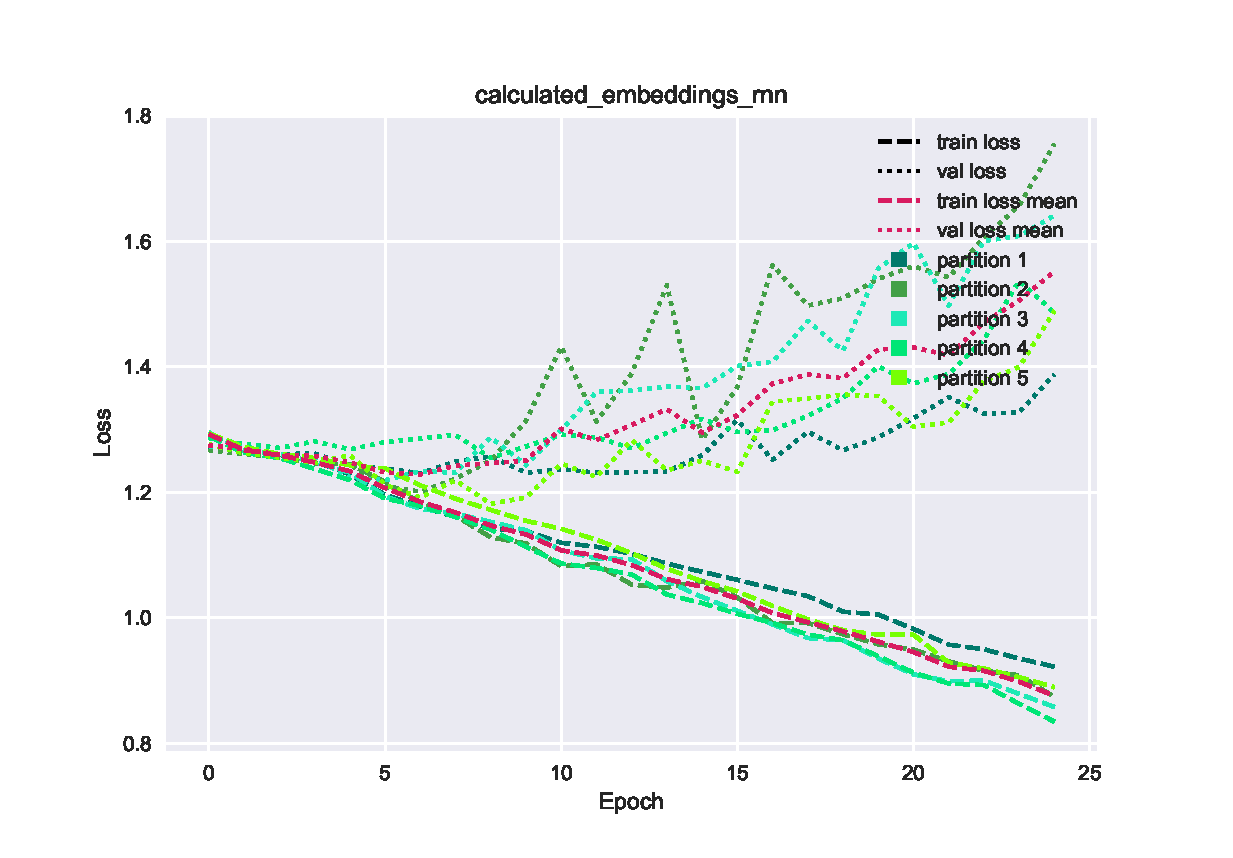
\includegraphics[width=\linewidth]{images/loss/calculated_embeddings_rnn-1554203049.eps}
\end{figure}

En este caso, el valor de la función \textit{loss} decrece según van pasando las épocas hasta la época cinco, pero luego se separa, sigue decreciendo para el conjunto de \textit{train} pero empieza a crecer para el conjunto de \textit{validation}. Esta situación nos indica que la red está sobreaprendiendo, tal y como hemos explicado anteriormente. Veamos ahora la arquitectura de la red:

\begin{verbatim}
Layer (type)                 Output Shape              Param #   
=================================================================
embedding_1 (Embedding)      (None, 35, 100)           499000    
lstm_2 (LSTM)                (None, 35, 64)            42240     
dense_3 (Dense)              (None, 35, 32)            2080      
flatten_2 (Flatten)          (None, 1120)              0         
dense_4 (Dense)              (None, 4)                 4484      
=================================================================
Total params: 547,804
Trainable params: 48,804
Non-trainable params: 499,000
\end{verbatim}

En este caso, no todos los parámetros de la red son entrenables. Si nos fijamos en el \textit{summary} de la arquitectura de la red, los parámetros no entrenables se encuentran en la capa de \textit{Embedding}, tal y como se ha comentado en la introducción a esta sección. Los resultados de este experimento son: 

\begin{table}[H]
\begin{tabular}{c|c|c}
\textbf{macro\_f1:} 0.283373 & \textbf{micro\_f1:} 0.433367 & \textbf{kaggle:} 0.45342
\end{tabular}
\end{table}

\subsection{pretrain\_embeddings\_rnn.} \label{exp_pretrainembeddingsrnn}

Experimento generado usando la red descrita en la sección \textit{pretrain\_embeddings\_rnn} (\ref{pretrainembeddingsrnn}) usando los parámetros por defecto indicados en la misma.

\begin{figure}[H]
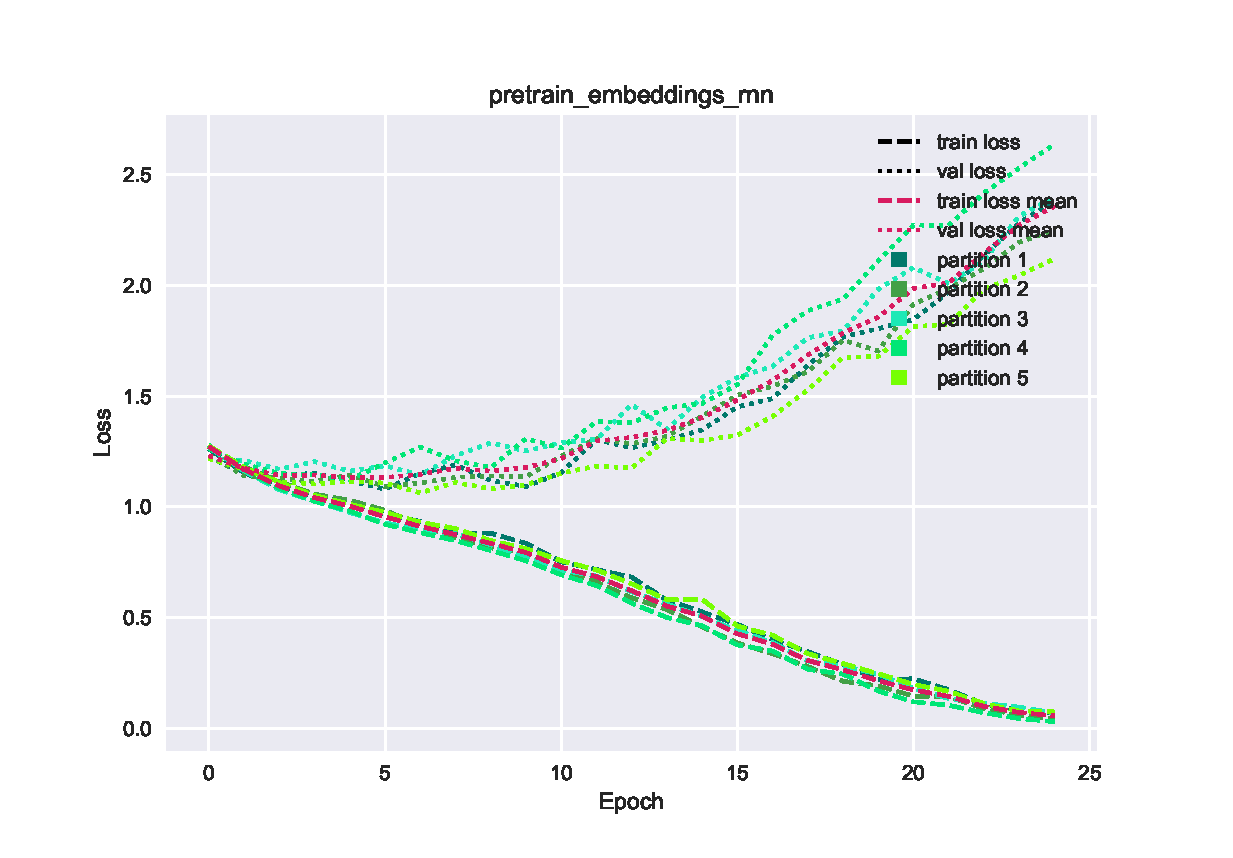
\includegraphics[width=\linewidth]{images/loss/pretrain_embeddings_rnn-1554203298.eps}
\end{figure}

En este caso, el valor de la función \textit{loss} decrece según van pasando las épocas hasta la época cinco, pero luego se separa, sigue decreciendo para el conjunto de \textit{train} pero empieza a crecer para el conjunto de \textit{validation}. Esta situación nos indica que la red está sobreaprendiendo, es decir, se hace muy buena en el conjunto de \textit{train} pero, cuando la enfrentas a datos nuevos, el resultado es bastante peor. Veamos ahora la arquitectura de la red:

\begin{verbatim}
Layer (type)                 Output Shape              Param #   
=================================================================
embedding_2 (Embedding)      (None, 16, 100)           51334200  
lstm_3 (LSTM)                (None, 16, 64)            42240     
dense_5 (Dense)              (None, 16, 32)            2080      
flatten_3 (Flatten)          (None, 512)               0         
dense_6 (Dense)              (None, 4)                 2052      
=================================================================
Total params: 51,380,572
Trainable params: 46,372
Non-trainable params: 51,334,200
\end{verbatim}

En este caso, no todos los parámetros de la red son entrenables. Si nos fijamos en el \textit{summary} de la arquitectura de la red, los parámetros no entrenables se encuentran en la capa de \textit{Embedding}, tal y como se ha comentado en la introducción a esta sección. En este caso, el número de parámetros no entrenados es mucho mayor ya que el conjunto de \textit{embeddings} se le proporciona a la red y es bastante mayor del calculado por la red en el experimento anterior. Los resultados de este experimento son: 

\begin{table}[H]
\begin{tabular}{c|c|c}
\textbf{macro\_f1:} 0.417279 & \textbf{micro\_f1:} 0.507906 & \textbf{kaggle:} 0.49384
\end{tabular}
\end{table}

\subsection{sigmoid\_pretrain\_embeddings\_rnn.} \label{exp_sigmoidpretrainembeddingsrnn}

Experimento generado usando la red descrita en la sección \textit{sigmoid\_pretrain\_embeddings\_rnn} (\ref{sigmoidpretrainembeddingsrnn}) usando los parámetros por defecto indicados en la misma.

\begin{figure}[H]
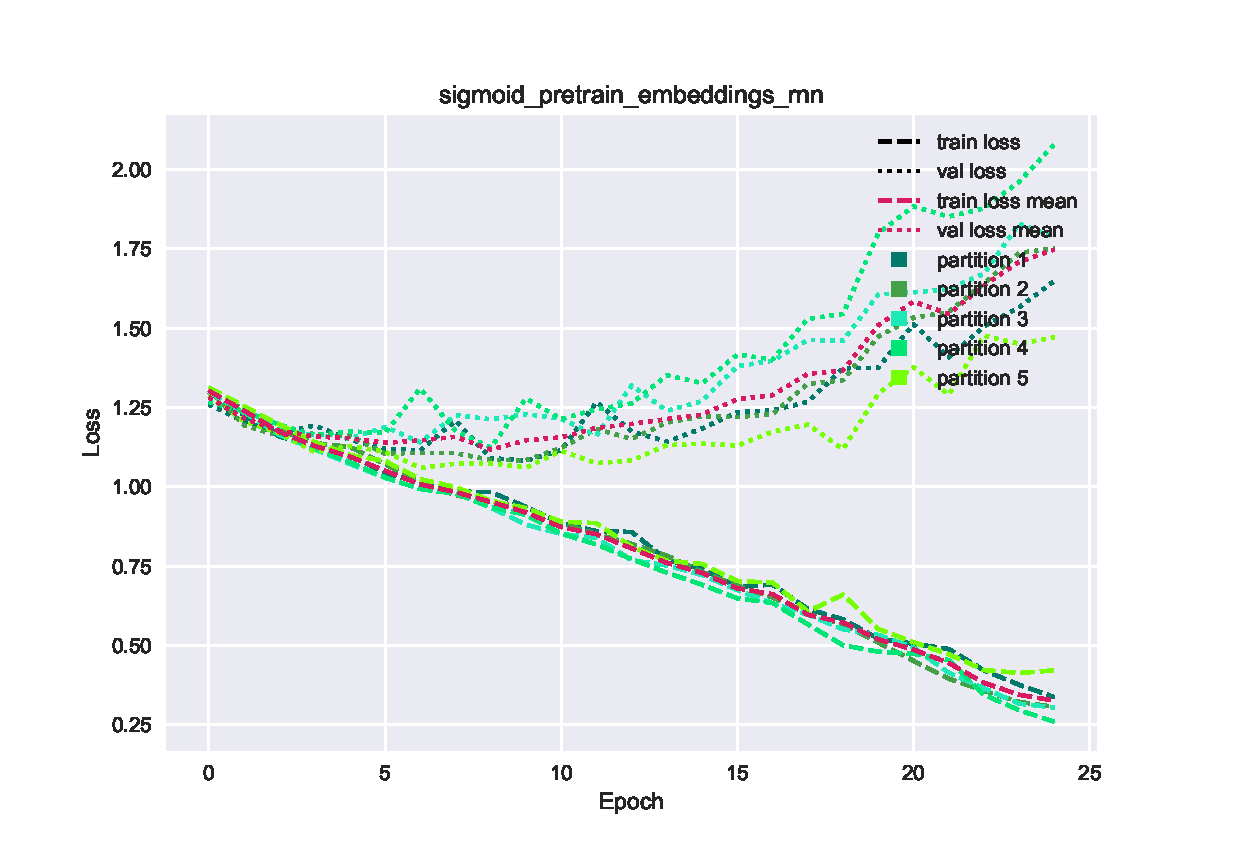
\includegraphics[width=\linewidth]{images/loss/sigmoid_pretrain_embeddings_rnn-1554203570.eps}
\end{figure}

Al igual que en el experimento anterior, el valor de la función \textit{loss} decrece según van pasando las épocas hasta la época cinco, pero luego se separa, sigue decreciendo para el conjunto de \textit{train} pero empieza a crecer para el conjunto de \textit{validation}, lo que nos indica que la red está sobreaprendiendo. Sin embargo, si nos fijamos en la escala sobre la que se mueven los valores de la función \textit{loss}, podemos ver que es menor, lo cual nos indica que la red está sobreaprendiendo menos que en el experimento anterior. Veamos ahora la arquitectura de la red:

\begin{verbatim}
Layer (type)                 Output Shape              Param #   
=================================================================
embedding_3 (Embedding)      (None, 16, 100)           51334200  
lstm_4 (LSTM)                (None, 16, 64)            42240     
dense_7 (Dense)              (None, 16, 32)            2080      
flatten_4 (Flatten)          (None, 512)               0         
dense_8 (Dense)              (None, 4)                 2052      
=================================================================
Total params: 51,380,572
Trainable params: 46,372
Non-trainable params: 51,334,200
\end{verbatim}

Una vez más, no todos los parámetros de la red son entrenables pero los parámetros no entrenables se encuentran en la capa de \textit{Embedding}. Los resultados de este experimento son: 

\begin{table}[H]
\begin{tabular}{c|c|c}
\textbf{macro\_f1:} 0.408407 & \textbf{micro\_f1:} 0.506601 & \textbf{kaggle:} 0.49560
\end{tabular}
\end{table}

\subsection{epochs100\_pretrain\_embeddings\_rnn.} \label{exp_epochs100pretrainembeddingsrnn}

Experimento generado usando la red descrita en la sección \textit{pretrain\_embeddings\_rnn} (\ref{pretrainembeddingsrnn}) usando los parámetros por defecto indicados en la misma. La diferencia con el experimento \textit{pretrain\_embeddings\_rnn} (\ref{exp_pretrainembeddingsrnn}) es que el número de épocas se ha incrementado hasta 100.

\begin{figure}[H]
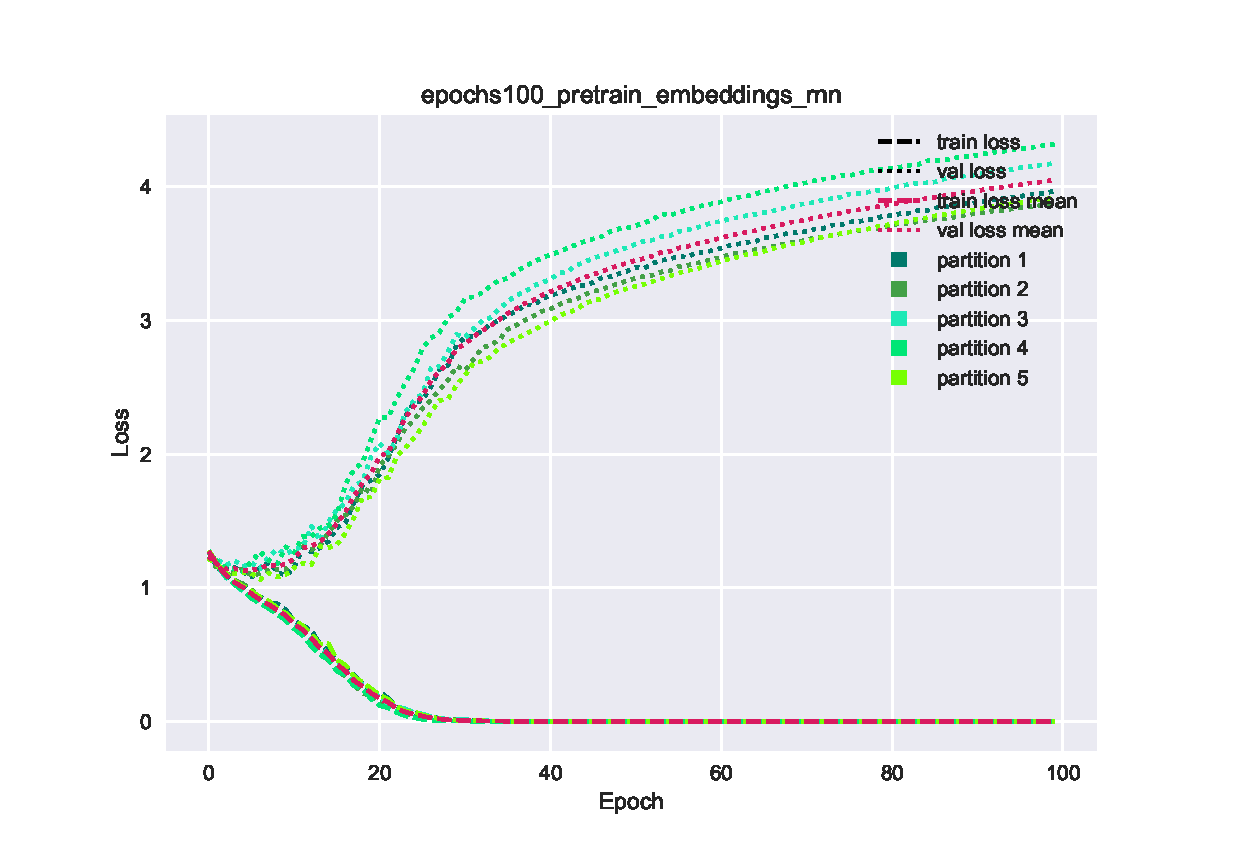
\includegraphics[width=\linewidth]{images/loss/epochs100_pretrain_embeddings_rnn-1554204046.eps}
\end{figure}

Si la red ya sobreaprendía con 25 épocas, podemos ver que con 100 épocas el sobreaprendizaje es bastante mayor. Veamos ahora la arquitectura de la red:

\begin{verbatim}
Layer (type)                 Output Shape              Param #   
=================================================================
embedding_4 (Embedding)      (None, 16, 100)           51334200  
lstm_5 (LSTM)                (None, 16, 64)            42240     
dense_9 (Dense)              (None, 16, 32)            2080      
flatten_5 (Flatten)          (None, 512)               0         
dense_10 (Dense)             (None, 4)                 2052      
=================================================================
Total params: 51,380,572
Trainable params: 46,372
Non-trainable params: 51,334,200
\end{verbatim}

Como en los experimentos anteriores, no todos los parámetros de la red son entrenables y esto se debe a los \textit{embeddings}. Los resultados de este experimento son: 

\begin{table}[H]
\begin{tabular}{c|c|c}
\textbf{macro\_f1:} 0.430359 & \textbf{micro\_f1:} 0.516541 & \textbf{kaggle:} 0.49560
\end{tabular}
\end{table}

\subsection{stacked\_lstm\_rnn.} \label{exp_stackedlstmrnn}

Experimento generado usando la red descrita en la sección \textit{stacked\_lstm\_rnn} (\ref{stackedlstmrnn}), usando los parámetros por defecto indicados en la misma.

\begin{figure}[H]
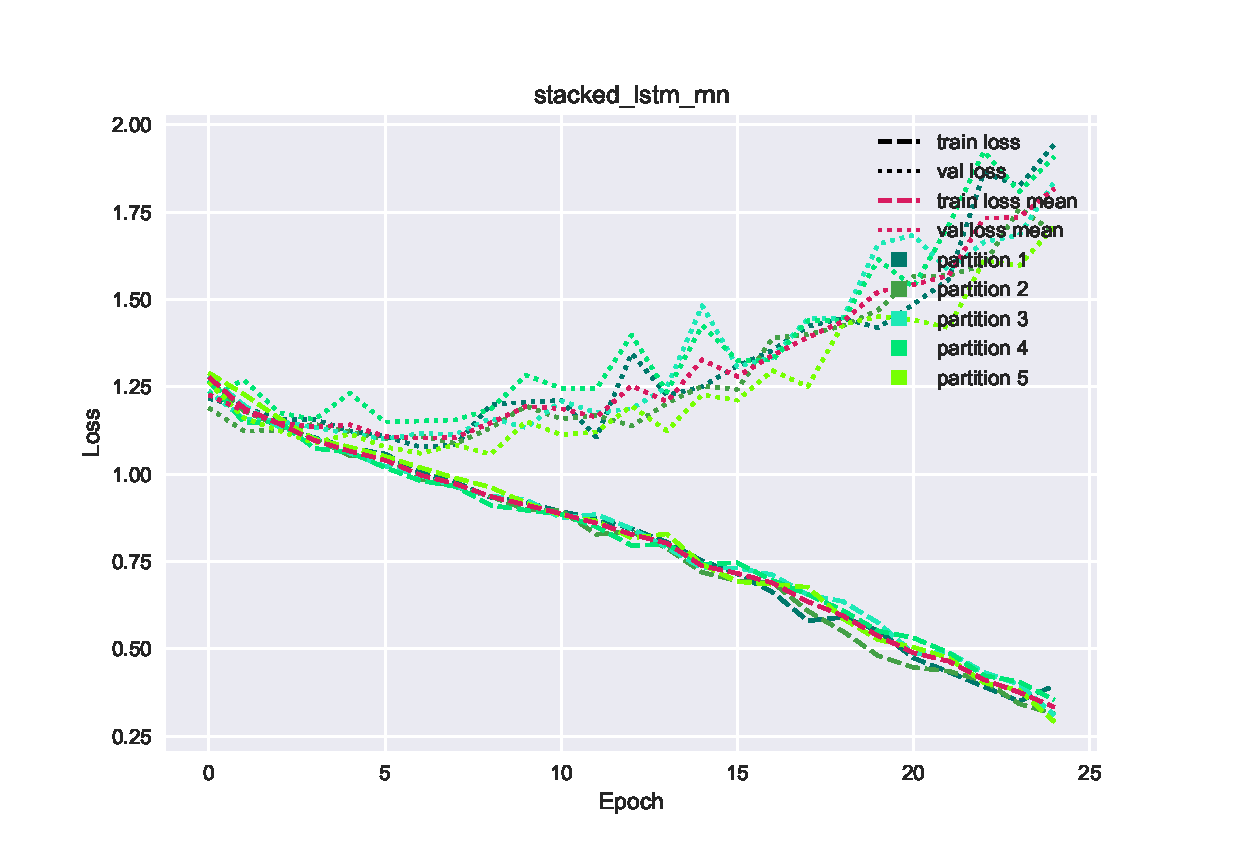
\includegraphics[width=\linewidth]{images/loss/stacked_lstm_rnn-1554204631.eps}
\end{figure}

Al igual que en los experimento anteriores, podemos apreciar que la red sobreaprende. Veamos ahora la arquitectura de la red:

\begin{verbatim}
Layer (type)                 Output Shape              Param #   
=================================================================
embedding_5 (Embedding)      (None, 16, 100)           51334200  
lstm_6 (LSTM)                (None, 16, 64)            42240     
lstm_7 (LSTM)                (None, 16, 64)            33024     
lstm_8 (LSTM)                (None, 16, 64)            33024     
lstm_9 (LSTM)                (None, 64)                33024     
dense_11 (Dense)             (None, 4)                 260       
=================================================================
Total params: 51,475,772
Trainable params: 141,572
Non-trainable params: 51,334,200
\end{verbatim}

Como en los experimentos anteriores, no todos los parámetros de la red son entrenables y esto se debe a los \textit{embeddings}. Los resultados de este experimento son: 

\begin{table}[H]
\begin{tabular}{c|c|c}
\textbf{macro\_f1:} 0.434354 & \textbf{micro\_f1:} 0.531007 & \textbf{kaggle:} 0.52372
\end{tabular}
\end{table}

\subsection{adadelta\_rnn.} \label{exp_adadeltarnn}

Experimento generado usando la red descrita en la sección \textit{adadelta\_rnn} (\ref{adadeltarnn}), usando los parámetros por defecto indicados en la misma.

\begin{figure}[H]
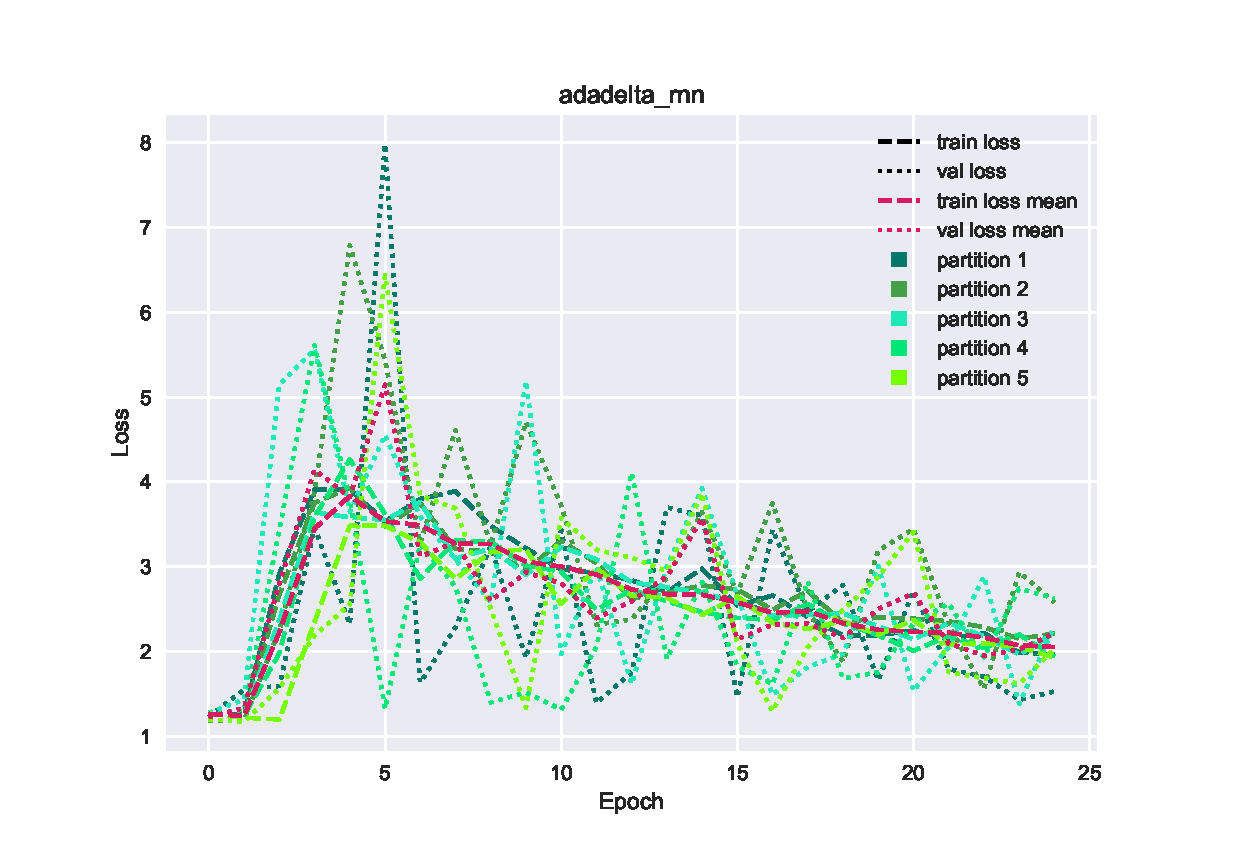
\includegraphics[width=\linewidth]{images/loss/adadelta_rnn-1554205042.eps}
\end{figure}

En este caso, no podemos decir que la red sobreaprenda ya que los valores de la función \textit{loss} para el conjunto de \textit{train} y el conjunto de \textit{validation} evolucionan de forma similar con el paso de las épocas. Veamos ahora la arquitectura de la red:

\begin{verbatim}
Layer (type)                 Output Shape              Param #   
=================================================================
embedding_1 (Embedding)      (None, 16, 100)           51334200  
lstm_1 (LSTM)                (None, 16, 64)            42240     
dense_1 (Dense)              (None, 16, 32)            2080      
flatten_1 (Flatten)          (None, 512)               0         
dense_2 (Dense)              (None, 4)                 2052      
=================================================================
Total params: 51,380,572
Trainable params: 46,372
Non-trainable params: 51,334,200
\end{verbatim}

Como en los experimentos anteriores, no todos los parámetros de la red son entrenables y esto se debe a los \textit{embeddings}. Los resultados de este experimento son: 

\begin{table}[H]
\begin{tabular}{c|c|c}
\textbf{macro\_f1:} 0.100923 & \textbf{micro\_f1:} 0.262983 & \textbf{kaggle:} No entregado
\end{tabular}
\end{table}

\subsection{adam\_lr\_0005\_rnn.} \label{exp_adamlr0005rnn}

Experimento generado usando la red descrita en la sección \textit{pretrain\_embeddings\_rnn} (\ref{pretrainembeddingsrnn}). En este caso, se ha cambiado el \textit{lerning rate} para que sea de \textit{0.005}.

\begin{figure}[H]
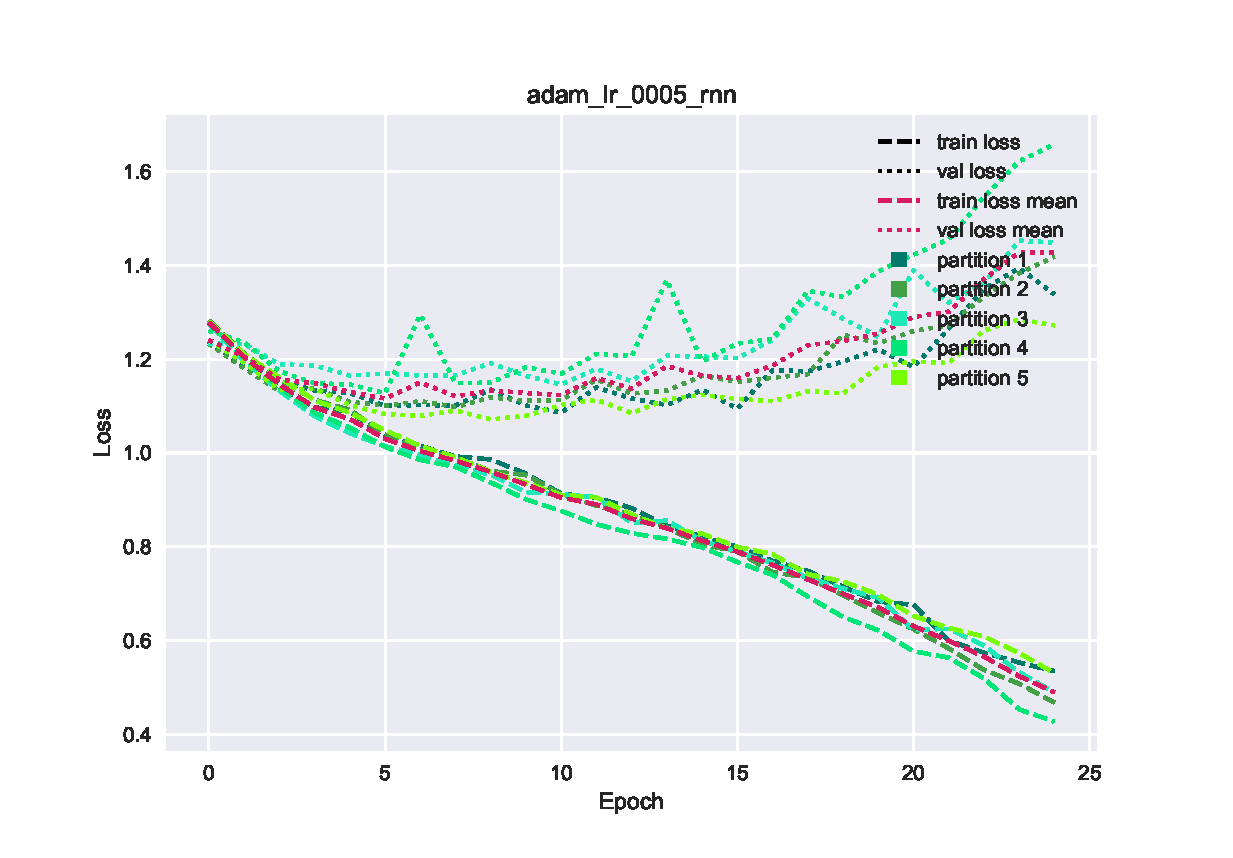
\includegraphics[width=\linewidth]{images/loss/adam_lr_0005_rnn-1554205482.eps}
\end{figure}

El \textit{learning rate} indica como de rápido aprende la red. Ya que hemos indicado un valor más alto, la red aprende más lento y, por lo tanto, no sobreaprende tanto como en los ejemplos anteriores, ya que no tiene tiempo (épocas) para hacerlo. Veamos ahora la arquitectura de la red:

\begin{verbatim}
Layer (type)                 Output Shape              Param #   
=================================================================
embedding_7 (Embedding)      (None, 16, 100)           51334200  
lstm_14 (LSTM)               (None, 16, 64)            42240     
dense_13 (Dense)             (None, 16, 32)            2080      
flatten_6 (Flatten)          (None, 512)               0         
dense_14 (Dense)             (None, 4)                 2052      
=================================================================
Total params: 51,380,572
Trainable params: 46,372
Non-trainable params: 51,334,200
\end{verbatim}

Como en los experimentos anteriores, no todos los parámetros de la red son entrenables y esto se debe a los \textit{embeddings}. Los resultados de este experimento son: 

\begin{table}[H]
\begin{tabular}{c|c|c}
\textbf{macro\_f1:} 0.424711 & \textbf{micro\_f1:} 0.526395 & \textbf{kaggle:} 0.50439
\end{tabular}
\end{table}

\subsection{pretrain\_embeddings\_LSTM\_CONV.} \label{exp_pretrainembeddingsLSTMCONV}

Experimento generado usando la red descrita en la sección \textit{pretrain\_embeddings\_LSTM\_CONV} (\ref{pretrainembeddingsLSTMCONV}), usando los parámetros por defecto indicados en la misma.

\begin{figure}[H]
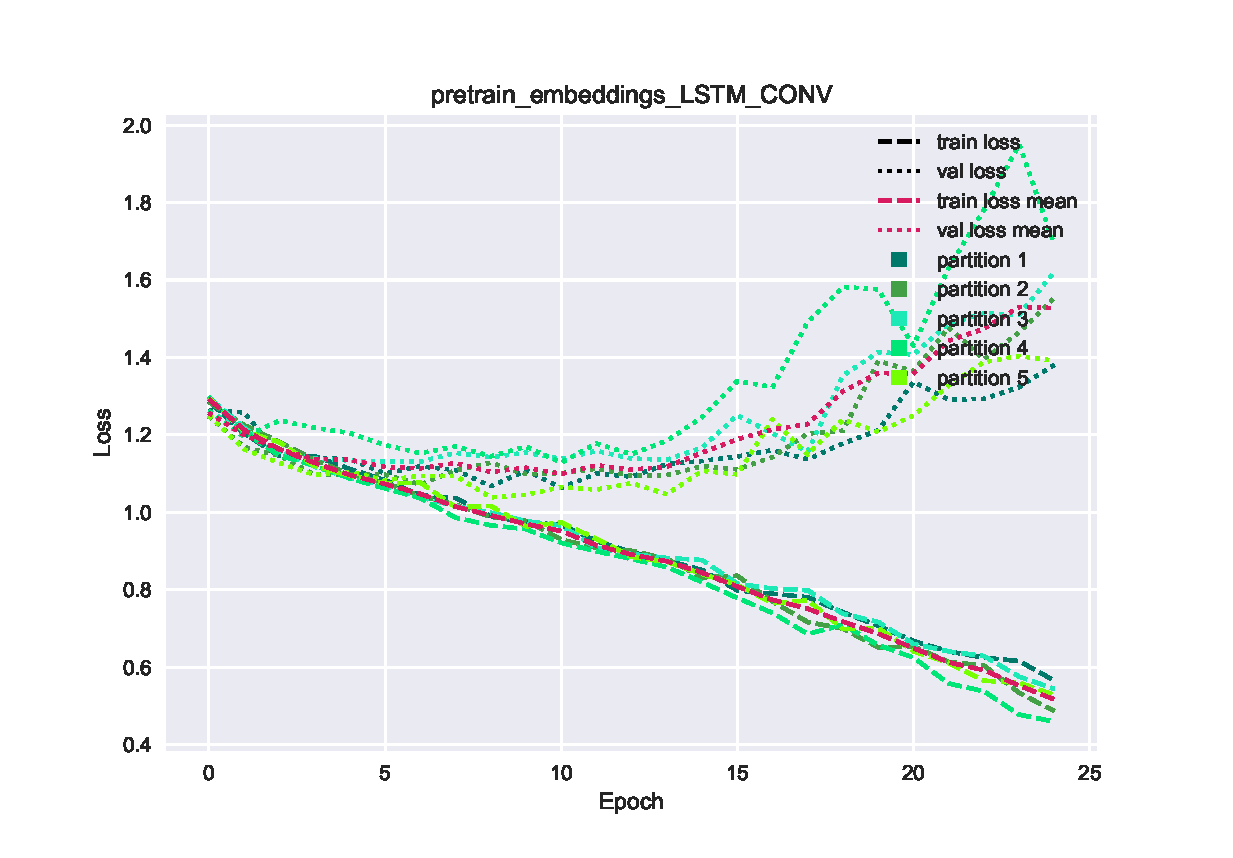
\includegraphics[width=\linewidth]{images/loss/pretrain_embeddings_LSTM_CONV-1554205954.eps}
\end{figure}

Al igual que en los experimento anteriores, podemos apreciar que la red sobreaprende. Veamos ahora la arquitectura de la red:

\begin{verbatim}
Layer (type)                 Output Shape              Param #   
=================================================================
embedding_8 (Embedding)      (None, 16, 100)           51334200  
lstm_15 (LSTM)               (None, 16, 64)            42240     
dropout_1 (Dropout)          (None, 16, 64)            0         
max_pooling1d_1 (MaxPooling1 (None, 8, 64)             0         
conv1d_1 (Conv1D)            (None, 8, 128)            41088     
dropout_2 (Dropout)          (None, 8, 128)            0         
average_pooling1d_1 (Average (None, 4, 128)            0         
dense_15 (Dense)             (None, 4, 128)            16512     
dropout_3 (Dropout)          (None, 4, 128)            0         
average_pooling1d_2 (Average (None, 2, 128)            0         
flatten_7 (Flatten)          (None, 256)               0         
dense_16 (Dense)             (None, 4)                 1028      
=================================================================
Total params: 51,435,068
Trainable params: 100,868
Non-trainable params: 51,334,200
\end{verbatim}

Como en los experimentos anteriores, no todos los parámetros de la red son entrenables y esto se debe a los \textit{embeddings}. Los resultados de este experimento son: 

\begin{table}[H]
\begin{tabular}{c|c|c}
\textbf{macro\_f1:} 0.443507 & \textbf{micro\_f1:} 0.526316 & \textbf{kaggle:} 0.51845
\end{tabular}
\end{table}

\subsection{preprocess\_tfidf\_rnn.} \label{exp_preprocesstfidfrnn}

Experimento generado usando la red descrita en la sección \textit{tfidf\_rnn} (\ref{tfidfrnn}), usando los parámetros por defecto indicados en la misma. La diferencia es que se ha aplicado el preprocesamiento explicado en la sección \textit{Preprocesamiento} (\ref{preprocesamiento}), sin contar \textit{oversampling}.

\begin{figure}[H]
\includegraphics[width=\linewidth]{images/loss/preprocess_tfidf_rnn-1554206135.eps}
\end{figure}

Al igual que sucedía en el experimento \textit{tfdidf\_rnn} (\ref{exp_tfidfrnn}), esta red no sobreaprende, ya que el valor de la función \textit{loss} evoluciona de manera similar para el conjunto de \textit{train} y el conjunto \textit{validation}. Veamos ahora la arquitectura de la red:

\begin{verbatim}
Layer (type)                 Output Shape              Param #   
=================================================================
lstm_16 (LSTM)               (None, 20, 64)            16896     
dense_17 (Dense)             (None, 20, 32)            2080      
flatten_8 (Flatten)          (None, 640)               0         
dense_18 (Dense)             (None, 4)                 2564      
=================================================================
Total params: 21,540
Trainable params: 21,540
Non-trainable params: 0
\end{verbatim}

Como en los experimentos anteriores, no todos los parámetros de la red son entrenables y esto se debe a los \textit{embeddings}. Los resultados de este experimento son: 

\begin{table}[H]
\begin{tabular}{c|c|c}
\textbf{macro\_f1:} 0.148071 & \textbf{micro\_f1:} 0.420742 & \textbf{kaggle:} 0.42179
\end{tabular}
\end{table}

\subsection{preprocess\_calculated\_embeddings\_rnn.} \label{exp_preprocesscalculatedembeddingsrnn}

Experimento generado usando la red descrita en la sección \textit{calculated\_embeddings\_rnn} (\ref{calculatedembeddingsrnn}), usando los parámetros por defecto indicados en la misma. La diferencia es que se ha aplicado el preprocesamiento explicado en la sección \textit{Preprocesamiento} (\ref{preprocesamiento}), sin contar \textit{oversampling}.

\begin{figure}[H]
\includegraphics[width=\linewidth]{images/loss/preprocess_calculated_embeddings_rnn-1554206519.eps}
\end{figure}

Al igual que sucedía en el experimento \textit{calculated\_embeddings\_rnn} (\ref{exp_calculatedembeddingsrnn}), esta red sobreaprende. Veamos ahora la arquitectura de la red:

\begin{verbatim}
Layer (type)                 Output Shape              Param #   
=================================================================
embedding_9 (Embedding)      (None, 27, 100)           379000    
lstm_17 (LSTM)               (None, 27, 64)            42240     
dense_19 (Dense)             (None, 27, 32)            2080      
flatten_9 (Flatten)          (None, 864)               0         
dense_20 (Dense)             (None, 4)                 3460      
=================================================================
Total params: 426,780
Trainable params: 47,780
Non-trainable params: 379,000
\end{verbatim}

Como en los experimentos anteriores, no todos los parámetros de la red son entrenables y esto se debe a los \textit{embeddings}. Los resultados de este experimento son: 

\begin{table}[H]
\begin{tabular}{c|c|c}
\textbf{macro\_f1:} 0.256807 & \textbf{micro\_f1:} 0.372415 & \textbf{kaggle:} 0.41827
\end{tabular}
\end{table}

\subsection{preprocess\_pretrain\_embeddings\_rnn.} \label{exp_preprocesspretrainembeddingsrnn}

Experimento generado usando la red descrita en la sección \textit{pretrain\_embeddings\_rnn} (\ref{pretrainembeddingsrnn}), usando los parámetros por defecto indicados en la misma. La diferencia es que se ha aplicado el preprocesamiento explicado en la sección \textit{Preprocesamiento} (\ref{preprocesamiento}), sin contar \textit{oversampling}.

\begin{figure}[H]
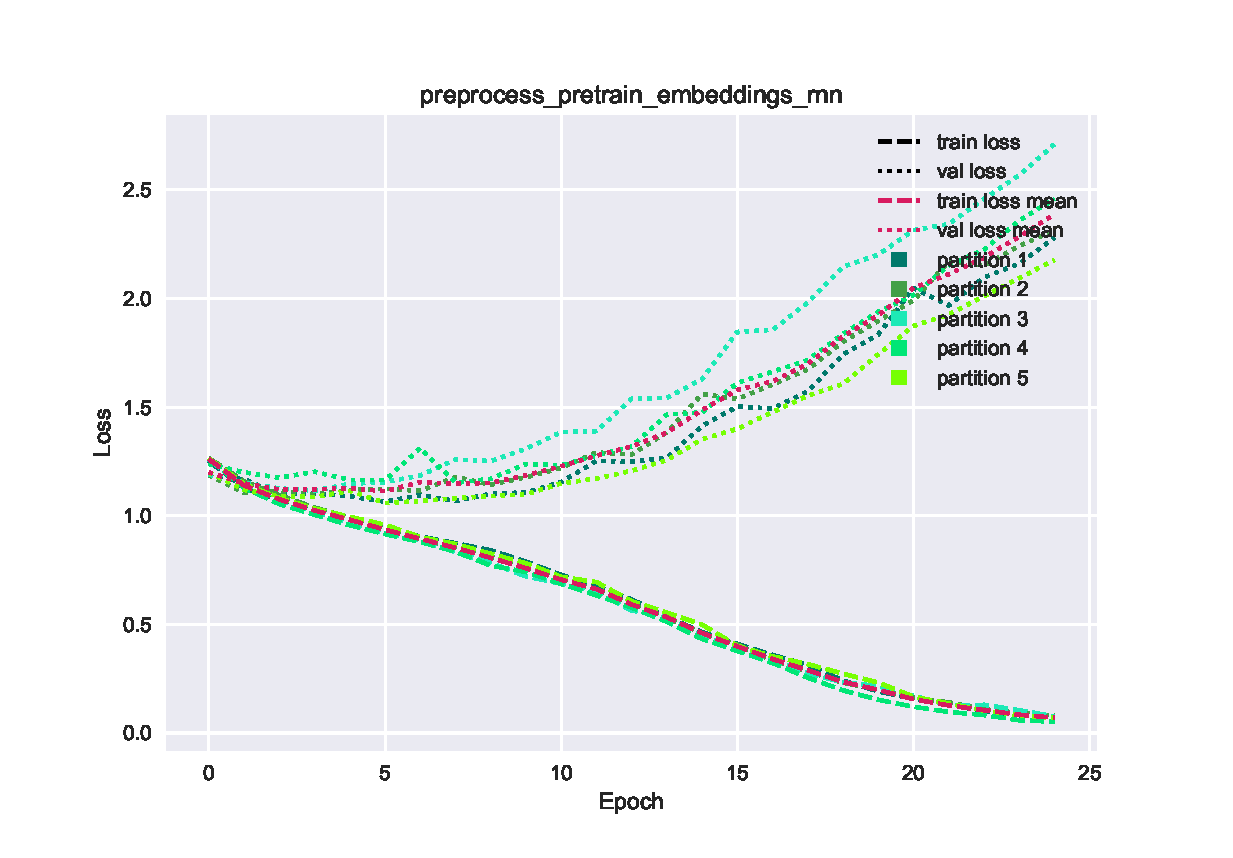
\includegraphics[width=\linewidth]{images/loss/preprocess_pretrain_embeddings_rnn-1554207097.eps}
\end{figure}

Al igual que sucedía en el experimento \textit{pretain\_embeddings\_rnn} (\ref{exp_pretrainembeddingsrnn}), esta red sobreaprende. Veamos ahora la arquitectura de la red:

\begin{verbatim}
Layer (type)                 Output Shape              Param #   
=================================================================
embedding_10 (Embedding)     (None, 9, 100)            51334200  
lstm_18 (LSTM)               (None, 9, 64)             42240     
dense_21 (Dense)             (None, 9, 32)             2080      
flatten_10 (Flatten)         (None, 288)               0         
dense_22 (Dense)             (None, 4)                 1156      
=================================================================
Total params: 51,379,676
Trainable params: 45,476
Non-trainable params: 51,334,200
\end{verbatim}

Como en los experimentos anteriores, no todos los parámetros de la red son entrenables y esto se debe a los \textit{embeddings}. Los resultados de este experimento son: 

\begin{table}[H]
\begin{tabular}{c|c|c}
\textbf{macro\_f1:} 0.416798 & \textbf{micro\_f1:} 0.50527 & \textbf{kaggle}: 0.50615
\end{tabular}
\end{table}

\subsection{preprocess\_calculated\_embeddings\_LSTM\_CONV.} \label{exp_preprocesscalculatedembeddingsLSTMCONV}

Experimento generado usando la red descrita en la sección \textit{calculated\_embeddings\_LSTM\_CONV} (\ref{calculatedembeddingsLSTMCONV}), usando los parámetros por defecto indicados en la misma. La diferencia es que se ha aplicado el preprocesamiento explicado en la sección \textit{Preprocesamiento} (\ref{preprocesamiento}), sin contar \textit{oversampling}.

\begin{figure}[H]
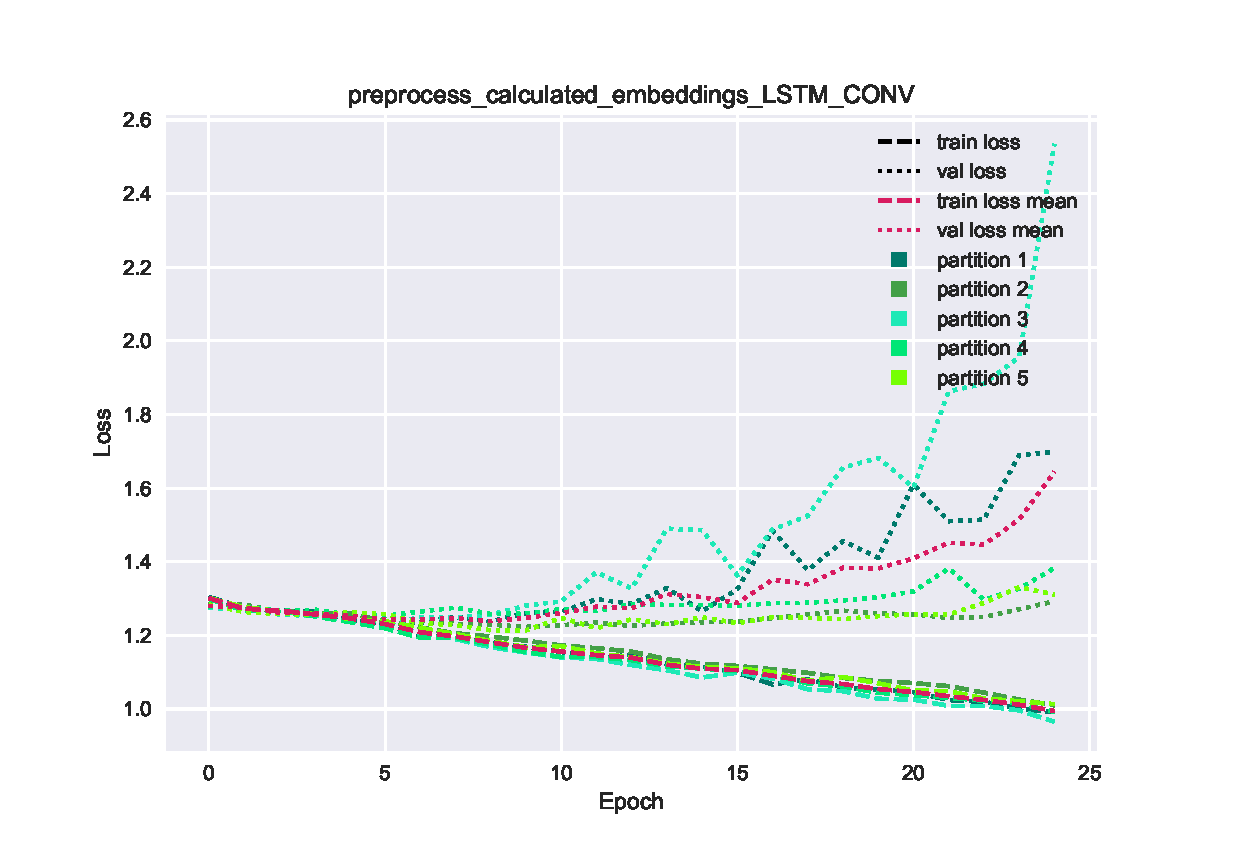
\includegraphics[width=\linewidth]{images/loss/preprocess_calculated_embeddings_LSTM_CONV-1554208275.eps}
\end{figure}

Como podemos ver, esta red sobreaprende, ya que el valor de la función \textit{loss} evoluciona de manera distinta para el conjunto de \textit{train} y el conjunto \textit{validation}, despuntándose incluso en una partición (la 3) a unos valores bastante más altos. Veamos ahora la arquitectura de la red:

\begin{verbatim}
Layer (type)                 Output Shape              Param #   
=================================================================
embedding_12 (Embedding)     (None, 27, 100)           379000    
lstm_20 (LSTM)               (None, 27, 64)            42240     
dropout_7 (Dropout)          (None, 27, 64)            0         
max_pooling1d_3 (MaxPooling1 (None, 13, 64)            0         
conv1d_3 (Conv1D)            (None, 13, 128)           41088     
dropout_8 (Dropout)          (None, 13, 128)           0         
average_pooling1d_5 (Average (None, 6, 128)            0         
dense_25 (Dense)             (None, 6, 128)            16512     
dropout_9 (Dropout)          (None, 6, 128)            0         
average_pooling1d_6 (Average (None, 3, 128)            0         
flatten_12 (Flatten)         (None, 384)               0         
dense_26 (Dense)             (None, 4)                 1540      
=================================================================
Total params: 480,380
Trainable params: 101,380
Non-trainable params: 379,000
\end{verbatim}

Como en los experimentos anteriores, no todos los parámetros de la red son entrenables y esto se debe a los \textit{embeddings}. Los resultados de este experimento son: 

\begin{table}[H]
\begin{tabular}{c|c|c}
\textbf{macro\_f1:} 0.260481 & \textbf{micro\_f1:} 0.450435 & \textbf{kaggle:} 0.36731
\end{tabular}
\end{table}

\subsection{epochs50\_preprocess\_calculated\_embeddings\_LSTM\_CONV.} \label{exp_epochs50preprocesscalculatedembeddingsLSTMCONV}

Este experimento es el mismo que el mostrado en la sección \textit{preprocess\_calculated\_embeddings\_LSTM\_CONV.} \ref{exp_preprocesscalculatedembeddingsLSTMCONV} pero con más épocas, \textit{50} en vez de \textit{25}. Hemos hecho este experimento para ver que sucedía con esa partición que despuntaba en las últimas épocas de aprendizaje.

\begin{figure}[H]
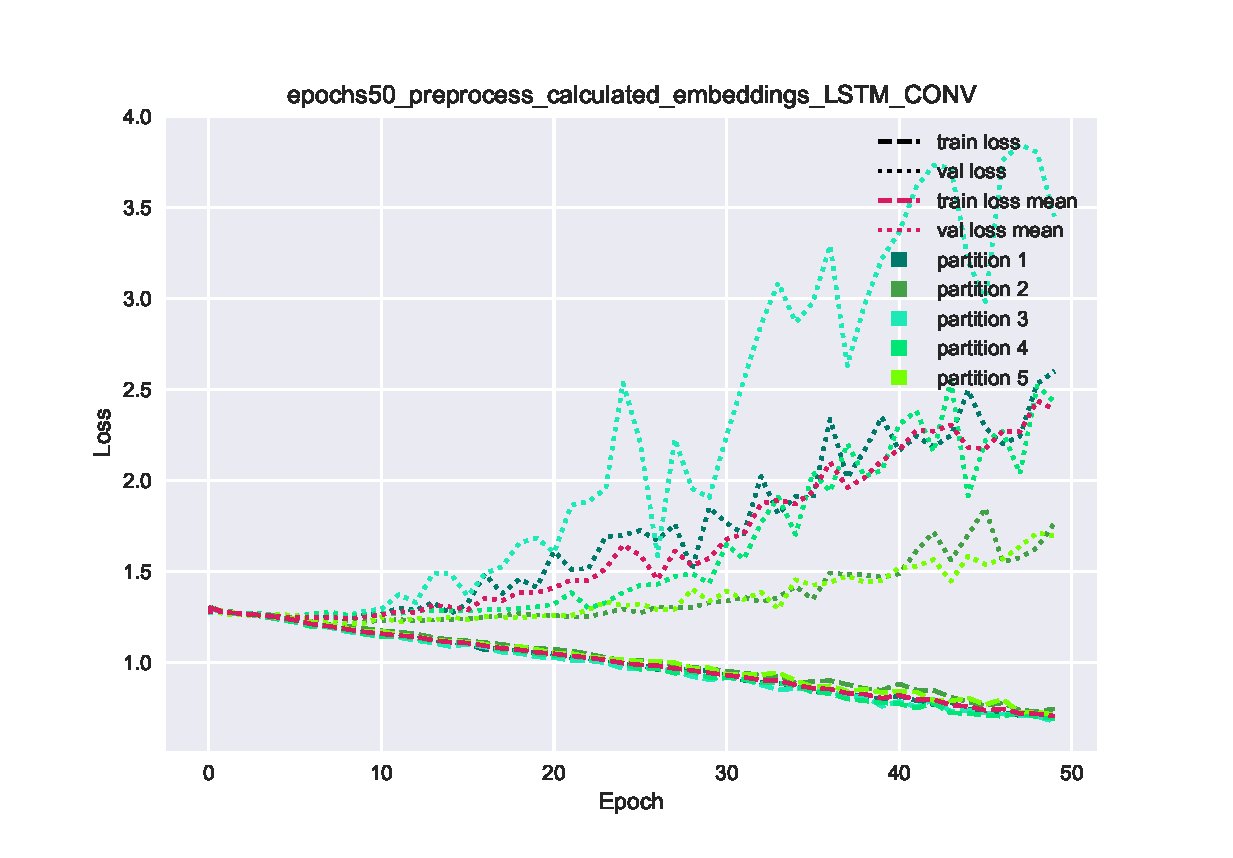
\includegraphics[width=\linewidth]{images/loss/epochs50_preprocess_calculated_embeddings_LSTM_CONV-1554208880.eps}
\end{figure}

Como podemos ver, el valor de la función \textit{loss} sigue creciendo conforme pasan las épocas y, por ello, aumenta el sobreaprendizaje de la red. Veamos ahora la arquitectura de la red:

\begin{verbatim}
Layer (type)                 Output Shape              Param #   
=================================================================
embedding_13 (Embedding)     (None, 27, 100)           379000    
lstm_21 (LSTM)               (None, 27, 64)            42240     
dropout_10 (Dropout)         (None, 27, 64)            0         
max_pooling1d_4 (MaxPooling1 (None, 13, 64)            0         
conv1d_4 (Conv1D)            (None, 13, 128)           41088     
dropout_11 (Dropout)         (None, 13, 128)           0         
average_pooling1d_7 (Average (None, 6, 128)            0         
dense_27 (Dense)             (None, 6, 128)            16512     
dropout_12 (Dropout)         (None, 6, 128)            0         
average_pooling1d_8 (Average (None, 3, 128)            0         
flatten_13 (Flatten)         (None, 384)               0         
dense_28 (Dense)             (None, 4)                 1540      
=================================================================
Total params: 480,380
Trainable params: 101,380
Non-trainable params: 379,000
\end{verbatim}

Como en los experimentos anteriores, no todos los parámetros de la red son entrenables y esto se debe a los \textit{embeddings}. Los resultados de este experimento son: 

\begin{table}[H]
\begin{tabular}{c|c|c}
\textbf{macro\_f1:} 0.297376 & \textbf{micro\_f1:} 0.418076 & \textbf{kaggle:} 0.36203
\end{tabular}
\end{table}

\subsection{preprocess\_pretrain\_embeddings\_LSTM\_CONV.} \label{exp_preprocesspretrainembeddingsLSTMCONV}

Experimento generado usando la red descrita en la sección \textit{pretrain\_embeddings\_LSTM\_CONV} (\ref{pretrainembeddingsLSTMCONV}), usando los parámetros por defecto indicados en la misma. La diferencia es que se ha aplicado el preprocesamiento explicado en la sección \textit{Preprocesamiento} (\ref{preprocesamiento}), sin contar \textit{oversampling}.

\begin{figure}[H]
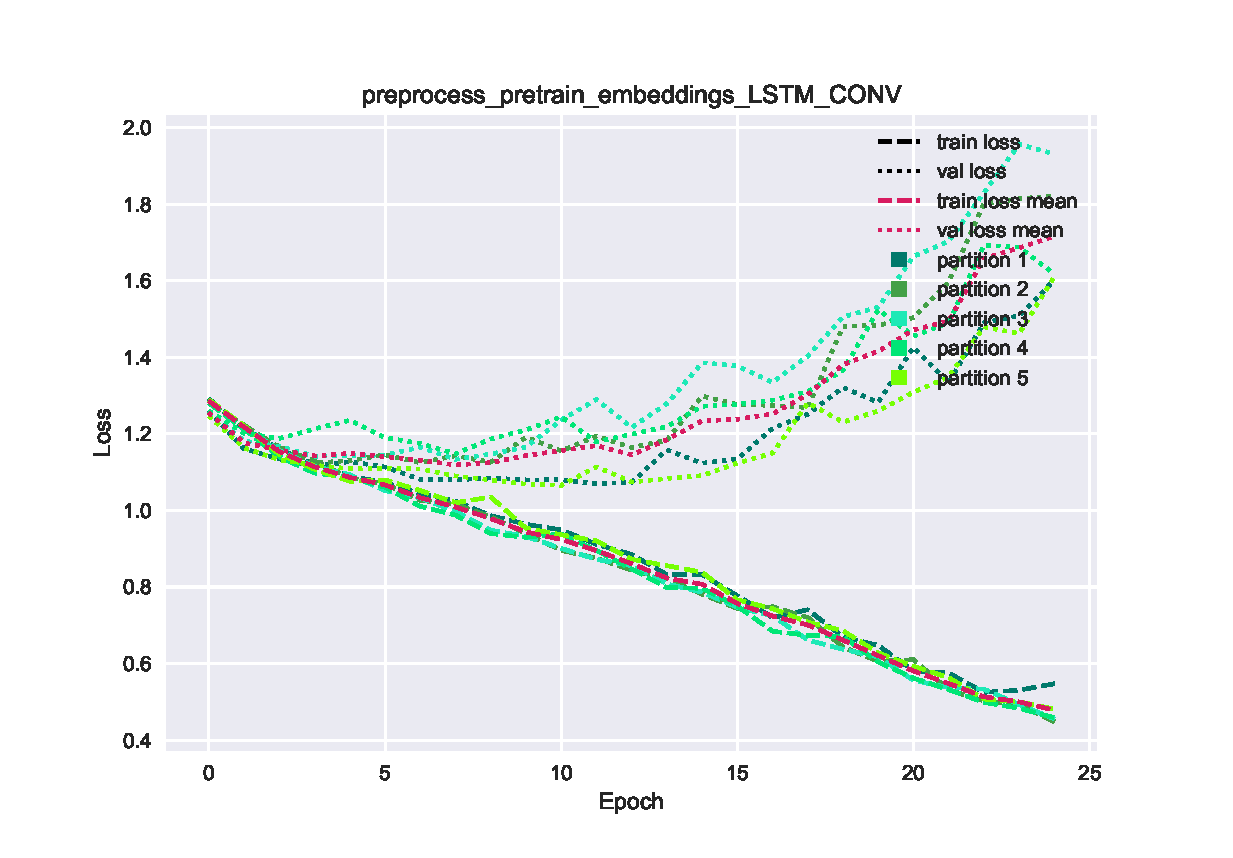
\includegraphics[width=\linewidth]{images/loss/preprocess_pretrain_embeddings_LSTM_CONV-1554207722.eps}
\end{figure}

Al igual que sucedía en el experimento \textit{pretrain\_embeddings\_LSTM\_CONV} (\ref{exp_pretrainembeddingsLSTMCONV}), esta red sobreaprende. Veamos ahora la arquitectura de la red:

\begin{verbatim}
Layer (type)                 Output Shape              Param #   
=================================================================
embedding_11 (Embedding)     (None, 9, 100)            51334200  
lstm_19 (LSTM)               (None, 9, 64)             42240     
dropout_4 (Dropout)          (None, 9, 64)             0         
max_pooling1d_2 (MaxPooling1 (None, 4, 64)             0         
conv1d_2 (Conv1D)            (None, 4, 128)            41088     
dropout_5 (Dropout)          (None, 4, 128)            0         
average_pooling1d_3 (Average (None, 2, 128)            0         
dense_23 (Dense)             (None, 2, 128)            16512     
dropout_6 (Dropout)          (None, 2, 128)            0         
average_pooling1d_4 (Average (None, 1, 128)            0         
flatten_11 (Flatten)         (None, 128)               0         
dense_24 (Dense)             (None, 4)                 516       
=================================================================
Total params: 51,434,556
Trainable params: 100,356
Non-trainable params: 51,334,200
\end{verbatim}

Como en los experimentos anteriores, no todos los parámetros de la red son entrenables y esto se debe a los \textit{embeddings}. Los resultados de este experimento son: 

\begin{table}[H]
\begin{tabular}{c|c|c}
\textbf{macro\_f1:} 0.418226 & \textbf{micro\_f1:} 0.48079 & \textbf{kaggle}: 0.50790
\end{tabular}
\end{table}

\subsection{big\_LSTM\_CONV\_rnn.} \label{exp_bigLSTMCONVrnn}

Experimento generado usando la red descrita en la sección \textit{big\_LSTM\_CONV\_rnn} (\ref{bigLSTMCONVrnn}), usando los parámetros por defecto indicados en la misma.

\begin{figure}[H]
\includegraphics[width=\linewidth]{images/loss/big_LSTM_CONV_rnn-1554209955.eps}
\end{figure}

Viendo la gráfica podemos ver que esta red sobreaprende, lo cual tiene sentido, ya que al aumentar el número de capas, la red es capaz de extraer conocimiento más específico y, por lo tanto, perder esa capacidad de generalización necesaria para clasificar correctamente nuevas instancias. Veamos ahora la arquitectura de la red:

\begin{verbatim}
Layer (type)                 Output Shape              Param #   
=================================================================
embedding_14 (Embedding)     (None, 9, 100)            51334200  
lstm_22 (LSTM)               (None, 9, 64)             42240     
dropout_13 (Dropout)         (None, 9, 64)             0         
conv1d_5 (Conv1D)            (None, 9, 128)            41088     
dropout_14 (Dropout)         (None, 9, 128)            0         
lstm_23 (LSTM)               (None, 9, 64)             49408     
dropout_15 (Dropout)         (None, 9, 64)             0         
conv1d_6 (Conv1D)            (None, 9, 128)            41088     
dropout_16 (Dropout)         (None, 9, 128)            0         
lstm_24 (LSTM)               (None, 9, 64)             49408     
dropout_17 (Dropout)         (None, 9, 64)             0         
conv1d_7 (Conv1D)            (None, 9, 128)            41088     
dropout_18 (Dropout)         (None, 9, 128)            0         
dense_29 (Dense)             (None, 9, 128)            16512     
dropout_19 (Dropout)         (None, 9, 128)            0         
flatten_14 (Flatten)         (None, 1152)              0         
dense_30 (Dense)             (None, 4)                 4612      
=================================================================
Total params: 51,619,644
Trainable params: 285,444
Non-trainable params: 51,334,200
\end{verbatim}

Como en los experimentos anteriores, no todos los parámetros de la red son entrenables y esto se debe a los \textit{embeddings}. Los resultados de este experimento son: 

\begin{table}[H]
\begin{tabular}{c|c|c}
\textbf{macro\_f1:} 0.413876 & \textbf{micro\_f1:} 0.553534 & \textbf{kaggle:} 0.30052
\end{tabular}
\end{table}

\subsection{dropout\_LSTM\_CONV\_rnn.} \label{exp_dropoutLSTMCONVrnn}

Experimento generado usando la red descrita en la sección \textit{dropout\_LSTM\_CONV\_rnn} (\ref{dropoutLSTMCONVrnn}), usando los parámetros por defecto indicados en la misma. 

\begin{figure}[H]
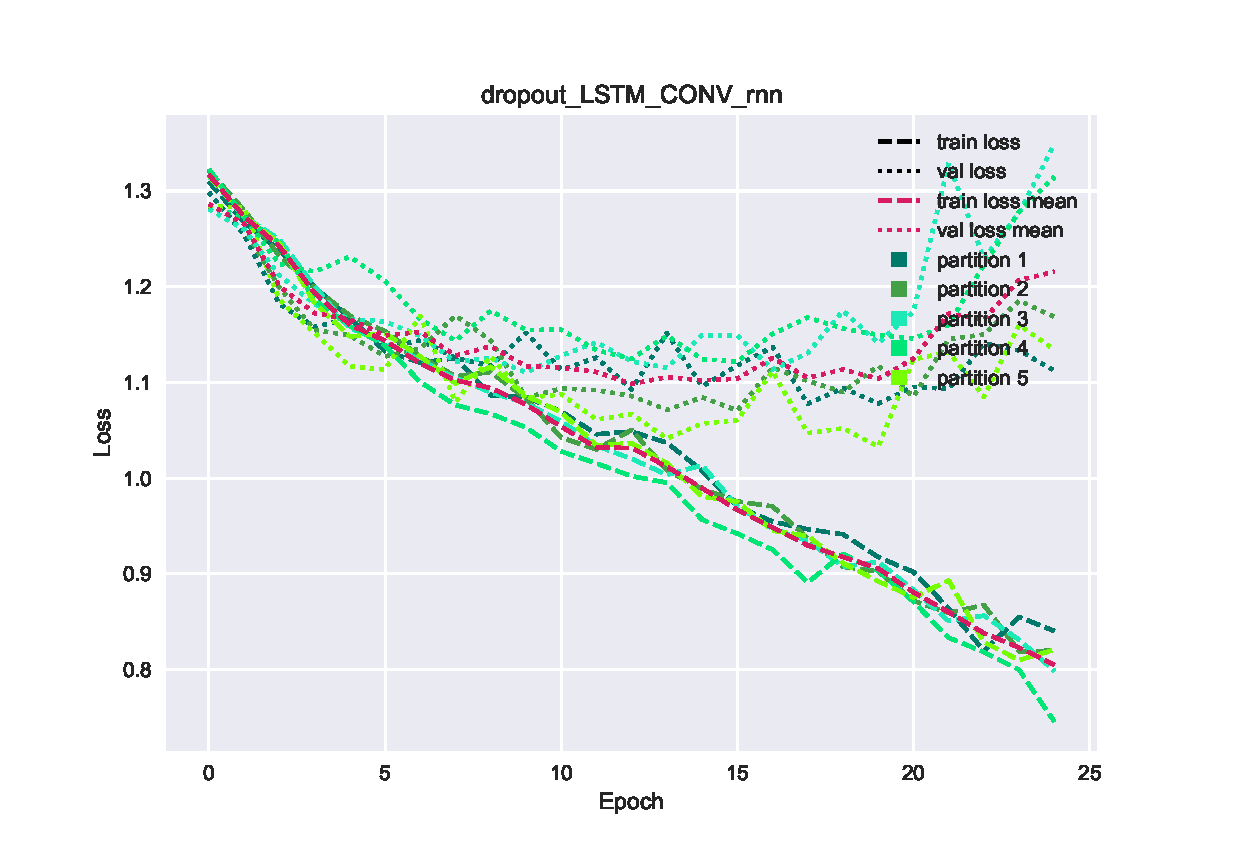
\includegraphics[width=\linewidth]{images/loss/dropout_LSTM_CONV_rnn-1554211023.eps}
\end{figure}

Si nos fijamos con detalle en esta gráfica podemos ver cierto parecido con la gráfica obtenida en el experimento \textit{adam\_lr\_0005} (\ref{exp_adamlr0005rnn}), ya que la red sobreaprende pero no tanto como en otros experimentos. Esto se debe a que, al haber introducido la técnica \textit{dropout}, hay neuronas que no aprenden en ciertas épocas, lo cual supone un aprendizaje de la red más lento, que es precisamento lo que se ha buscado en el experimento \textit{adam\_lr\_0005} (\ref{exp_adamlr0005rnn}) aumentando el \textit{learning\_rate}. Veamos ahora la arquitectura de la red:

\begin{verbatim}
Layer (type)                 Output Shape              Param #   
=================================================================
embedding_15 (Embedding)     (None, 16, 100)           51334200  
lstm_25 (LSTM)               (None, 16, 64)            42240     
dropout_20 (Dropout)         (None, 16, 64)            0         
max_pooling1d_5 (MaxPooling1 (None, 8, 64)             0         
conv1d_8 (Conv1D)            (None, 8, 128)            41088     
dropout_21 (Dropout)         (None, 8, 128)            0         
average_pooling1d_9 (Average (None, 4, 128)            0         
dense_31 (Dense)             (None, 4, 128)            16512     
dropout_22 (Dropout)         (None, 4, 128)            0         
average_pooling1d_10 (Averag (None, 2, 128)            0         
flatten_15 (Flatten)         (None, 256)               0         
dense_32 (Dense)             (None, 4)                 1028      
=================================================================
Total params: 51,435,068
Trainable params: 100,868
Non-trainable params: 51,334,200
\end{verbatim}

Como en los experimentos anteriores, no todos los parámetros de la red son entrenables y esto se debe a los \textit{embeddings}. Los resultados de este experimento son: 

\begin{table}[H]
\begin{tabular}{c|c|c}
\textbf{macro\_f1:} 0.432329 & \textbf{micro\_f1:} 0.554804 & \textbf{kaggle:} 0.54305
\end{tabular}
\end{table}

\subsection{pretrain\_embeddings\_LSTM\_CONV\_OVERSAMPLING.} \label{exp_pretrainembeddingsLSTMCONVOVERSAMPLING}

Experimento generado usando la red descrita en la sección \textit{pretrain\_embeddings\_LSTM\_CONV} (\ref{pretrainembeddingsLSTMCONV}), usando los parámetros por defecto indicados en la misma. La diferencia es que se ha aplicado \textit{oversampling}, tal y cómo se ha explicado en la sección \textit{Preprocesamiento} (\ref{preprocesamiento}).

\begin{figure}[H]
\includegraphics[width=\linewidth]{images/loss/pretrain_embeddings_LSTM_CONV_OVERSAMPLING-1554388456.eps}
\end{figure}

Al igual que sucedía en el experimento \textit{pretrain\_embeddings\_LSTM\_CONV} (\ref{exp_pretrainembeddingsLSTMCONV}), esta red sobreaprende, pero de una manera más irregular (obsérvese los valores de la función \textit{loss} para las particiones del conjunto \textit{validation} -las líneas de puntos-). Veamos ahora la arquitectura de la red:

\begin{verbatim}
Layer (type)                 Output Shape              Param #   
=================================================================
embedding_1 (Embedding)      (None, 11, 100)           51334200  
lstm_1 (LSTM)                (None, 11, 64)            42240     
dropout_1 (Dropout)          (None, 11, 64)            0         
max_pooling1d_1 (MaxPooling1 (None, 5, 64)             0         
conv1d_1 (Conv1D)            (None, 5, 128)            41088     
dropout_2 (Dropout)          (None, 5, 128)            0         
average_pooling1d_1 (Average (None, 2, 128)            0         
dense_1 (Dense)              (None, 2, 128)            16512     
dropout_3 (Dropout)          (None, 2, 128)            0         
average_pooling1d_2 (Average (None, 1, 128)            0         
flatten_1 (Flatten)          (None, 128)               0         
dense_2 (Dense)              (None, 4)                 516       
=================================================================
Total params: 51,434,556
Trainable params: 100,356
Non-trainable params: 51,334,200
\end{verbatim}

Como en los experimentos anteriores, no todos los parámetros de la red son entrenables y esto se debe a los \textit{embeddings}. Los resultados de este experimento son: 

\begin{table}[H]
\begin{tabular}{c|c|c}
\textbf{macro\_f1:} 0.515203 & \textbf{micro\_f1:} 0.542741 & \textbf{kaggle:} 0.49912
\end{tabular}
\end{table}

\subsection{bidirectional\_lstm\_rnn.} \label{exp_bidirectionallstmrnn}

Experimento generado usando la red descrita en la sección \textit{bidirectional\_lstm\_rnn} (\ref{bidirectionallstmrnn}), usando los parámetros por defecto indicados en la misma. 

\begin{figure}[H]
\includegraphics[width=\linewidth]{images/loss/bidirectional_lstm_rnn-1554328051.eps}
\end{figure}

En este caso, los valores de la función \textit{loss} decrecen tanto en el conjunto de \textit{train} como en el conjunto de \textit{validation}, lo cual es la situación deseada, ya que nos indica que la red no sobreaprende. Veamos ahora la arquitectura de la red:

\begin{verbatim}
Layer (type)                 Output Shape              Param #   
=================================================================
embedding_16 (Embedding)     (None, 16, 100)           51334200  
bidirectional_1 (Bidirection (None, 16, 200)           160800    
global_max_pooling1d_1 (Glob (None, 200)               0         
dense_33 (Dense)             (None, 100)               20100     
dropout_23 (Dropout)         (None, 100)               0         
dense_34 (Dense)             (None, 4)                 404       
=================================================================
Total params: 51,515,504
Trainable params: 181,304
Non-trainable params: 51,334,200
\end{verbatim}

Como en los experimentos anteriores, no todos los parámetros de la red son entrenables y esto se debe a los \textit{embeddings}. Los resultados de este experimento son: 

\begin{table}[H]
\begin{tabular}{c|c|c}
\textbf{macro\_f1:} 0.392873 & \textbf{micro\_f1:} 0.561425 & \textbf{kaggle:} 0.57996
\end{tabular}
\end{table}

\subsection{fasttext\_sbwc\_bidirectional\_lstm\_rnn.} \label{exp_fasttextsbwcbidirectionallstmrnn}

Este experimento es el mismo que el mostrado en la sección \textit{bidirectional\_lstm\_rnn} (\ref{exp_bidirectionallstmrnn}) pero usando un conjunto distinto de \textit{embeddings}. En este primer ejemplo se han usado los \textit{embeddings} generados con \textit{FastText} (\href{https://github.com/facebookresearch/fastText}{https://github.com/facebookresearch/fastText}) usando el \textit{corpus} \textit{Spanish Billion Word Corpus} (\href{http://crscardellino.github.io/SBWCE/}{http://crscardellino.github.io/SBWCE/}).

\begin{figure}[H]
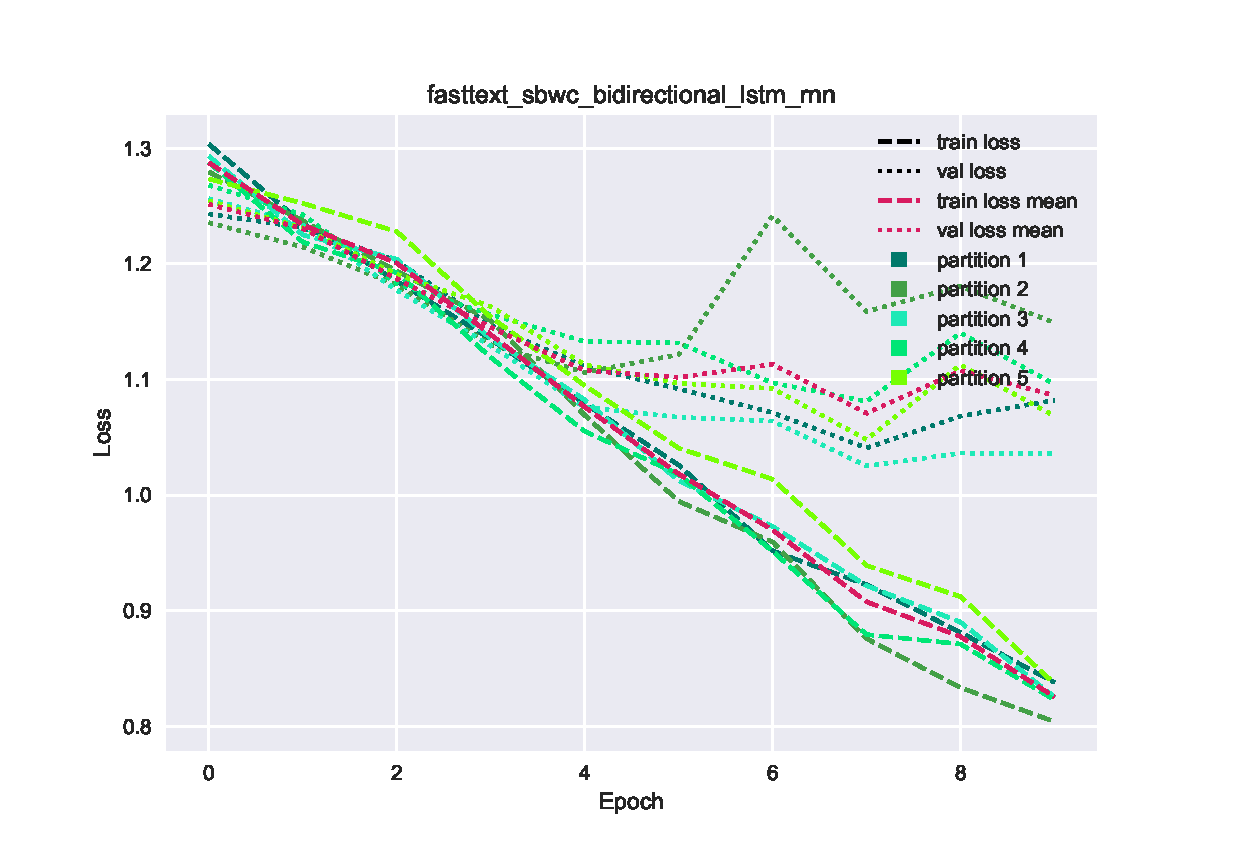
\includegraphics[width=\linewidth]{images/loss/fasttext_sbwc_bidirectional_lstm_rnn-1554399443.eps}
\end{figure}

Como podemos ver, en este caso si se produce sobreaprendizaje, lo cual nos hace ver la importancia de seleccionar unos buenos \textit{embeddings} para el problema que queremos resolver. Veamos ahora la arquitectura de la red:

\begin{verbatim}
Layer (type)                 Output Shape              Param #   
=================================================================
embedding_1 (Embedding)      (None, 16, 300)           256614600 
bidirectional_1 (Bidirection (None, 16, 200)           320800    
global_max_pooling1d_1 (Glob (None, 200)               0         
dense_1 (Dense)              (None, 100)               20100     
dropout_1 (Dropout)          (None, 100)               0         
dense_2 (Dense)              (None, 4)                 404       
=================================================================
Total params: 256,955,904
Trainable params: 341,304
Non-trainable params: 256,614,600
\end{verbatim}

Como en los experimentos anteriores, no todos los parámetros de la red son entrenables y esto se debe a los \textit{embeddings}. Sin embargo, podemos ver que el número de parámetros no entrenables en la capa \textit{Embedding} es mayor en comparación con el experimento original, ya que el tamaño del fichero de \textit{embeddings} es mayor. Los resultados de este experimento son: 

\begin{table}[H]
\begin{tabular}{c|c|c}
\textbf{macro\_f1:} 0.419309 & \textbf{micro\_f1:} 0.559381 & \textbf{kaggle:} 0.56414
\end{tabular}
\end{table}

\subsection{glove\_sbwc\_i25\_bidirectional\_lstm\_rnn.} \label{exp_glovesbwci25bidirectionallstmrnn}

Este experimento es el mismo que el mostrado en la sección \textit{bidirectional\_lstm\_rnn} (\ref{exp_bidirectionallstmrnn}) pero usando un conjunto distinto de \textit{embeddings}. En este primer ejemplo se han usado los \textit{embeddings} generados con \textit{GloVe} (\href{https://github.com/stanfordnlp/GloVe}{https://github.com/stanfordnlp/GloVe}) usando el \textit{corpus} \textit{Spanish Billion Word Corpus} (\href{http://crscardellino.github.io/SBWCE/}{http://crscardellino.github.io/SBWCE/}).

\begin{figure}[H]
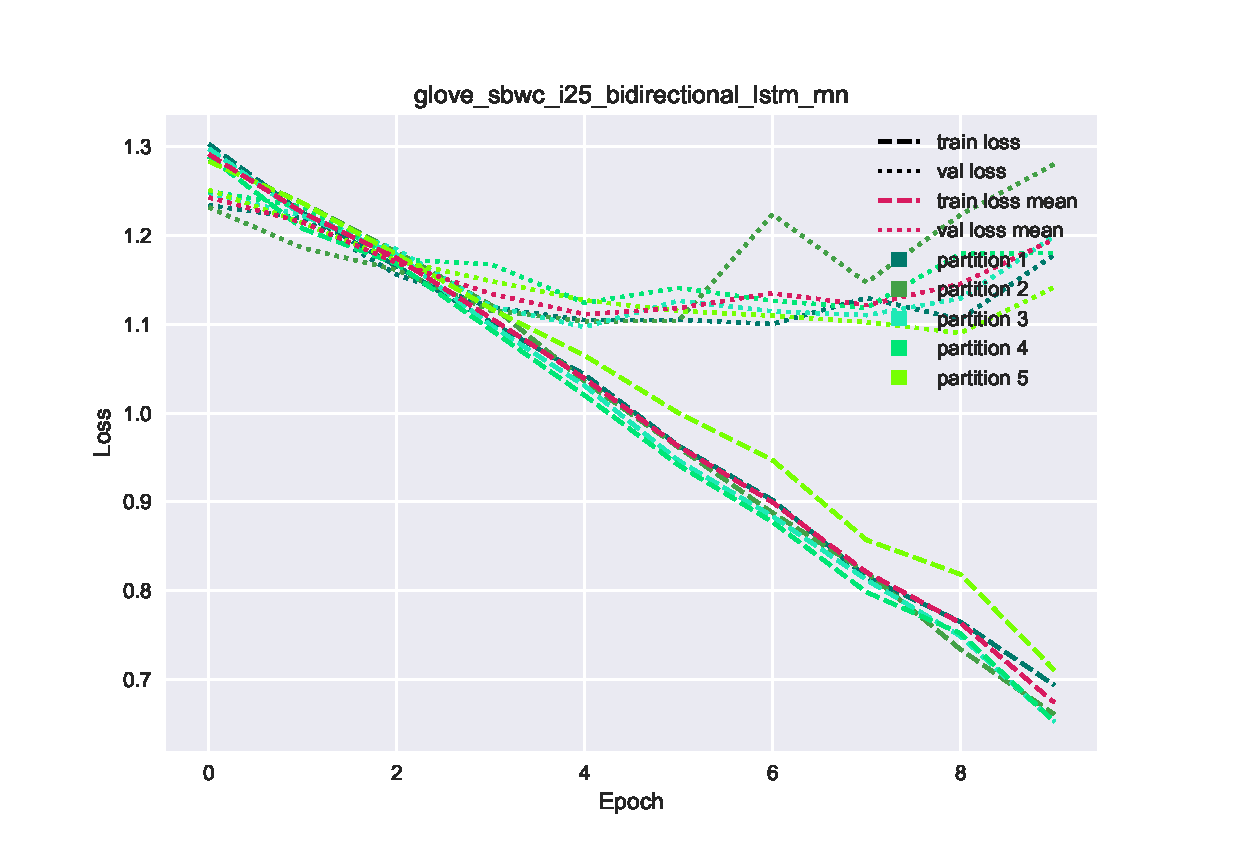
\includegraphics[width=\linewidth]{images/loss/glove_sbwc_i25_bidirectional_lstm_rnn-1554400692.eps}
\end{figure}

Como podemos ver, en este caso si se produce sobreaprendizaje, lo cual nos hace ver la importancia de seleccionar unos buenos \textit{embeddings} para el problema que queremos resolver. Veamos ahora la arquitectura de la red:

\begin{verbatim}
Layer (type)                 Output Shape              Param #   
=================================================================
embedding_1 (Embedding)      (None, 16, 300)           256614600 
bidirectional_1 (Bidirection (None, 16, 200)           320800    
global_max_pooling1d_1 (Glob (None, 200)               0         
dense_1 (Dense)              (None, 100)               20100     
dropout_1 (Dropout)          (None, 100)               0         
dense_2 (Dense)              (None, 4)                 404       
=================================================================
Total params: 256,955,904
Trainable params: 341,304
Non-trainable params: 256,614,600
\end{verbatim}

Como en los experimentos anteriores, no todos los parámetros de la red son entrenables y esto se debe a los \textit{embeddings}. Sin embargo, podemos ver que el número de parámetros no entrenables en la capa \textit{Embedding} es mayor en comparación con el experimento original, ya que el tamaño del fichero de \textit{embeddings} es mayor. Los resultados de este experimento son: 

\begin{table}[H]
\begin{tabular}{c|c|c}
\textbf{macro\_f1:} 0.435177 & \textbf{micro\_f1:} 0.534398 & \textbf{kaggle:} 0.55360
\end{tabular}
\end{table}

\subsection{SBW\_vectors\_300\_min5\_bidirectional\_lstm\_rnn.} \label{exp_SBWvectors300min5bidirectionallstmrnn}

Este experimento es el mismo que el mostrado en la sección \textit{bidirectional\_lstm\_rnn} (\ref{exp_bidirectionallstmrnn}) pero usando un conjunto distinto de \textit{embeddings}. En este primer ejemplo se han usado los \textit{embeddings} generados con \textit{Word2Vec} (\href{https://radimrehurek.com/gensim/models/word2vec.html}{https://radimrehurek.com/gensim/models/word2vec.html}) usando el \textit{corpus} \textit{Spanish Billion Word Corpus} (\href{http://crscardellino.github.io/SBWCE/}{http://crscardellino.github.io/SBWCE/}).

\begin{figure}[H]
\includegraphics[width=\linewidth]{images/loss/SBW_vectors_300_min5_bidirectional_lstm_rnn-1554402884.eps}
\end{figure}

En este caso, los valores de la función \textit{loss} decrecen tanto en el conjunto de \textit{train} como en el conjunto de \textit{validation}, lo cual es la situación deseada, ya que nos indica que la red no sobreaprende. Veamos ahora la arquitectura de la red:

\begin{verbatim}
Layer (type)                 Output Shape              Param #   
=================================================================
embedding_1 (Embedding)      (None, 16, 300)           300196500 
bidirectional_1 (Bidirection (None, 16, 200)           320800    
global_max_pooling1d_1 (Glob (None, 200)               0         
dense_1 (Dense)              (None, 100)               20100     
dropout_1 (Dropout)          (None, 100)               0         
dense_2 (Dense)              (None, 4)                 404       
=================================================================
Total params: 300,537,804
Trainable params: 341,304
Non-trainable params: 300,196,500
\end{verbatim}

Como en los experimentos anteriores, no todos los parámetros de la red son entrenables y esto se debe a los \textit{embeddings}. Sin embargo, podemos ver que el número de parámetros no entrenables en la capa \textit{Embedding} es mayor en comparación con el experimento original, ya que el tamaño del fichero de \textit{embeddings} es mayor. Los resultados de este experimento son: 

\begin{table}[H]
\begin{tabular}{c|c|c}
\textbf{macro\_f1:} 0.297016 & \textbf{micro\_f1:} 0.518501 & \textbf{kaggle:} 0.46572
\end{tabular}
\end{table}

\subsection{wiki\_es\_bidirectional\_lstm\_rnn.} \label{exp_wikiesbidirectionallstmrnn}

Este experimento es el mismo que el mostrado en la sección \textit{bidirectional\_lstm\_rnn} (\ref{exp_bidirectionallstmrnn}) pero usando un conjunto distinto de \textit{embeddings}. En este primer ejemplo se han usado los \textit{embeddings} generados con \textit{FastText} (\href{https://github.com/facebookresearch/fastText}{https://github.com/facebookresearch/fastText}) usando el \textit{corpus} \textit{Wikipedia Spanish Dump on January 05, 2015} (\href{https://archive.org/details/eswiki-20150105}{https://archive.org/details/eswiki-20150105}).

\begin{figure}[H]
\includegraphics[width=\linewidth]{images/loss/wiki_es_bidirectional_lstm_rnn-1554403834.eps}
\end{figure}

Como podemos ver, en este caso si se produce sobreaprendizaje, lo cual nos hace ver la importancia de seleccionar unos buenos \textit{embeddings} para el problema que queremos resolver. Veamos ahora la arquitectura de la red:

\begin{verbatim}
Layer (type)                 Output Shape              Param #   
=================================================================
embedding_7 (Embedding)      (None, 16, 300)           295700700 
bidirectional_7 (Bidirection (None, 16, 200)           320800    
global_max_pooling1d_7 (Glob (None, 200)               0         
dense_13 (Dense)             (None, 100)               20100     
dropout_7 (Dropout)          (None, 100)               0         
dense_14 (Dense)             (None, 4)                 404       
=================================================================
Total params: 296,042,004
Trainable params: 341,304
Non-trainable params: 295,700,700
\end{verbatim}

Como en los experimentos anteriores, no todos los parámetros de la red son entrenables y esto se debe a los \textit{embeddings}. Sin embargo, podemos ver que el número de parámetros no entrenables en la capa \textit{Embedding} es mayor en comparación con el experimento original, ya que el tamaño del fichero de \textit{embeddings} es mayor. Los resultados de este experimento son: 

\begin{table}[H]
\begin{tabular}{c|c|c}
\textbf{macro\_f1:} 0.427138 & \textbf{micro\_f1:} 0.530431 & \textbf{kaggle:} 0.56414
\end{tabular}
\end{table}

\subsection{pretrained\_embeddings\_cnn\_bidirectional\_LSTM.} \label{exp_pretrainedembeddingsbidirectionalLSTMCNNGRU}

Experimento generado usando la red descrita en la sección \textit{pretrained\_embeddings\_cnn\_bidirectional\_LSTM} (\ref{pretrainedembeddingscnnbidirectionalLSTM}), usando los parámetros por defecto indicados en la misma. 

\begin{figure}[H]
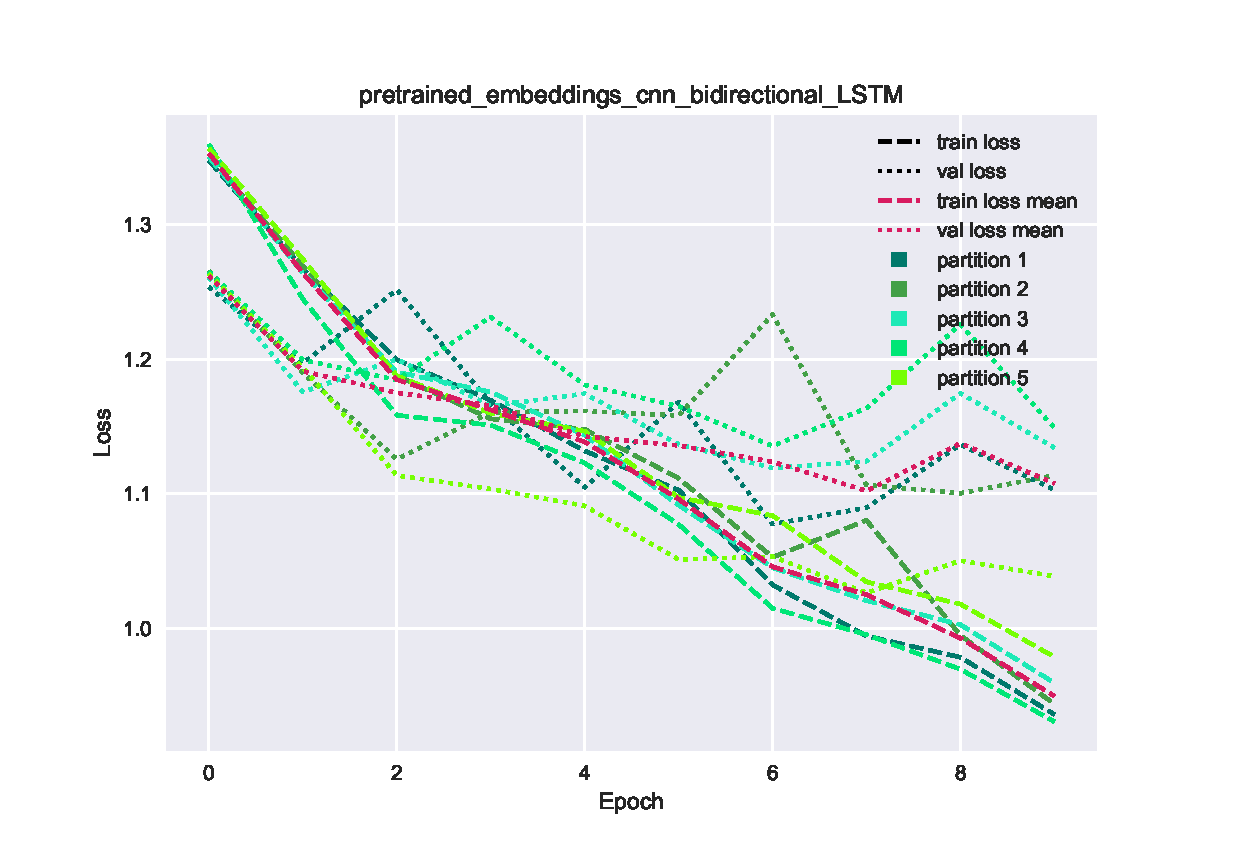
\includegraphics[width=\linewidth]{images/loss/pretrained_embeddings_cnn_bidirectional_LSTM-1554820745.eps}
\end{figure}

Como podemos ver esta red no sobreaprende demasiado, aunque parece que lo va a hacer si la hubiésemos dejado más épocas, ya que el valor de la función \textit{loss} empieza a separarse para el conjunto de \textit{validation} con respecto al conjunto de \textit{train}. Veamos ahora la arquitectura de la red:

\begin{verbatim}
************* pretrained_embeddings_cnn_bidirectional_LSTM *************
Layer (type)                 Output Shape              Param #   
=================================================================
embedding_1 (Embedding)      (None, 16, 100)           51334200  
conv1d_1 (Conv1D)            (None, 16, 64)            32064     
dropout_1 (Dropout)          (None, 16, 64)            0         
average_pooling1d_1 (Average (None, 8, 64)             0         
bidirectional_1 (Bidirection (None, 8, 600)            876000    
max_pooling1d_1 (MaxPooling1 (None, 4, 600)            0         
dense_1 (Dense)              (None, 4, 100)            60100     
dropout_2 (Dropout)          (None, 4, 100)            0         
average_pooling1d_2 (Average (None, 2, 100)            0         
flatten_1 (Flatten)          (None, 200)               0         
dense_2 (Dense)              (None, 4)                 804       
=================================================================
Total params: 52,303,168
Trainable params: 968,968
Non-trainable params: 51,334,200
\end{verbatim}

Como en los experimentos anteriores, no todos los parámetros de la red son entrenables y esto se debe a los \textit{embeddings}. Sin embargo, podemos ver, esta es la red con el mayor número de parámetros entrenables de los experimentos realizados. Los resultados de este experimento son: 

\begin{table}[H]
\begin{tabular}{c|c|c}
\textbf{macro\_f1:} 0.391742 & \textbf{micro\_f1:} 0.557514 & \textbf{kaggle:} 0.58347
\end{tabular}
\end{table}

\section{Otros experimentos.}

\subsection{Variables calculadas.}

Después de haber probado el enfoque conocido para el análisis de texto y que se basa en la conversión de las palabras de un texto en números utilizando maneras diferentes como vimos en nuestros experimentos ya explicados antes, hemos intentado transformar el conjunto de \textit{tuits} en un dataset que tiene un concepto y arquitectura totalmente diferente al original. Para ello hemos estudiado las características que creemos que pueden representar a un \textit{tuit}, en nuestro caso estas características son: \\

\begin{itemize}
    \item Longitud de texto.
    \item Número de palabras que refieren a duda o interrogación.
    \item Número de \textit{hashtags}.
    \item Número de palabras con letras repetidas más de 2 veces.
    \item Si el texto tiene o no signos de interrogación y/o signos de exclamación.
    \item Número de palabras que refieren a insultos o sentimientos negativos. Para ello, hemos definido una lista de los mismos.
    \item Cálculo de un factor de negatividad que se relaciona con el factor comentado en el punto anterior y el número total de palabras del texto.
    \item Número de palabras que refieren a sentimiento positivo.
    \item Cálculo de un factor de positividad que se relaciona con el factor comentado en el punto anterior y el número total de palabras del texto.
\end{itemize}
    
Pero al contrario de lo esperado, éste modelo de dataset no nos guiaba a modelos potentes, sino a modelos con una precisión muy baja en comparación a los obtenidos anteriormente.

\subsection{GRU.}

Los experimentos que se han hecho con \textit{GRU}, no daban una mejora sobre \textit{LSTM} y esto se puede entender por la demostración de \textit{Gail Weiss \& Yoav Goldberg \& Eran Yahav} (\href{https://arxiv.org/abs/1805.04908}{https://arxiv.org/abs/1805.04908}), la cual indica que \textit{LSTM} es ``estrictamente más fuerte'' que \textit{GRU}, ya que puede realizar fácilmente el conteo ilimitado, mientras que \textit{GRU} no puede. Es por eso que \textit{GRU} no aprende idiomas simples que se pueden aprender con \textit{LSTM}. \\

La unidad \textit{GRU} controla el flujo de información como la unidad \textit{LSTM}, pero sin tener que usar una unidad de memoria. Simplemente expone el contenido oculto completo sin ningún control. \textit{GRU} es relativamente nuevo, y la única ventaja que puede tener sobre \textit{LSTM} es en tema de eficiencia computacional.

\section{Resultados.}

A continuación, mostramos una tabla resumen de todos los resultados mostrados en esta memoria. Dicha tabla tiene los modelos ordenados en base a su puntuación obtenida en \textit{Kaggle}. Los tres modelos seleccionados para la entrega han sido los tres primeros de esta tabla.

\begin{sidewaystable}[htbp]
\medskip
\resizebox{\linewidth}{!}{%
\tabcolsep=2pt
\begin{tabular}{rcccrrr}
\multicolumn{1}{l}{} & \multicolumn{1}{l}{} & \multicolumn{1}{l}{} & \multicolumn{1}{l}{} & \multicolumn{3}{c}{\textbf{Número de parámetros}} \\ \cline{5-7} 
\multicolumn{1}{l}{} & \multicolumn{1}{l}{} & \multicolumn{1}{l}{} & \multicolumn{1}{l}{} & \multicolumn{1}{l}{\textbf{}} & \multicolumn{2}{c}{\textbf{¿Entrenables?}} \\ \cline{6-7} 
 & \textbf{macro\_f1} & \textbf{micro\_f1} & \textbf{kaggle} & \multicolumn{1}{c}{\textbf{Total}} & \multicolumn{1}{c}{\textbf{No}} & \multicolumn{1}{c}{\textbf{Si}} \\ \hline
\textbf{pretrained\_embeddings\_cnn\_bidirectional\_LSTM} & 0.391742 & 0.557514 & 0.58347 & 52,303,168 & 51,334,200 & 968,968 \\
\textbf{bidirectional\_lstm\_rnn\_results} & 0.392873 & 0.561425 & 0.57996 & 51,515,504 & 51,334,200 & 181,304 \\
\textbf{fasttext\_sbwc\_bidirectional\_lstm\_rnn} & 0.419309 & 0.559381 & 0.56414 & 256,955,904 & 256,614,600 & 341,304 \\
\textbf{wiki\_es\_bidirectional\_lstm\_rnn} & 0.427138 & 0.530431 & 0.56414 & 296,042,004 & 295,700,700 & 341,304 \\
\textbf{glove\_sbwc\_i25\_bidirectional\_lstm\_rnn} & 0.435177 & 0.534398 & 0.5536 & 256,955,904 & 256,614,600 & 341,304 \\
\textbf{dropout\_LSTM\_CONV\_rnn} & 0.432329 & 0.554804 & 0.54305 & 51,334,200 & 51,435,068 & 100,868 \\
\textbf{stacked\_lstm\_rnn} & 0.434354 & 0.531007 & 0.52372 & 51,475,772 & 51,334,200 & 141,572 \\
\textbf{pretrain\_embeddings\_LSTM\_CONV} & 0.443507 & 0.526316 & 0.51845 & 51,435,068 & 51,334,200 & 100,868 \\
\textbf{preprocess\_pretrain\_embeddings\_LSTM\_CONV} & 0.418226 & 0.480790 & 0.50790 & 51,434,556 & 51,334,200 & 100,356 \\
\textbf{preprocess\_pretrain\_embeddings\_rnn} & 0.416798 & 0.505270 & 0.50615 & 51,379,676 & 51,334,200 & 45,476 \\
\textbf{adam\_lr\_0005\_rnn} & 0.424711 & 0.526395 & 0.50439 & 51,380,572 & 51,334,200 & 46,372 \\
\textbf{pretrain\_embeddings\_LSTM\_CONV\_OVERSAMPLING} & 0.515203 & 0.542741 & 0.49912 & 51,434,556 & 51,334,200 & 100,356 \\
\textbf{epochs100\_pretrain\_embeddings\_rnn} & 0.430359 & 0.516541 & 0.49560 & 51,380,572 & 51,334,200 & 46,372 \\
\textbf{sigmoid\_pretrain\_embeddings\_rnn} & 0.408407 & 0.506601 & 0.49560 & 51,380,572 & 51,334,200 & 46,372 \\
\textbf{pretrain\_embeddings\_rnn} & 0.417279 & 0.507906 & 0.49384 & 51,380,572 & 51,334,200 & 46,372 \\
\textbf{SBW\_vectors\_300\_min5\_bidirectional\_lstm\_rnn} & 0.297016 & 0.518501 & 0.46572 & 300,537,804 & 300,196,500 & 341,304 \\
\textbf{calculated\_embeddings\_rnn} & 0.283373 & 0.433367 & 0.45342 & 499,000 & 547,804 & 48,804 \\
\textbf{preprocess\_tfidf\_rnn} & 0.148071 & 0.420742 & 0.42179 & 21,540 & 0 & 21,540 \\
\textbf{tfidf\_rnn} & 0.159393 & 0.414133 & 0.42179 & 22,692 & 0 & 22,692 \\
\textbf{preprocess\_calculated\_embeddings\_rnn} & 0.256807 & 0.372415 & 0.41827 & 426,780 & 379,000 & 47,780 \\
\textbf{preprocess\_calculated\_embeddings\_LSTM\_CONV} & 0.260481 & 0.450435 & 0.36731 & 480,380 & 379,000 & 101,380 \\
\textbf{epochs50\_preprocess\_calculated\_embeddings\_LSTM\_CONV} & 0.297376 & 0.418076 & 0.36203 & 480,380 & 379,000 & 101,380 \\
\textbf{big\_LSTM\_CONV\_rnn} & 0.413876 & 0.553534 & 0.30052 & 51,619,644 & 51,334,200 & 285,444 \\
\textbf{adadelta\_rnn} & 0.100923 & 0.262983 & \_ & 51,380,572 & 51,334,200 & 46,372
\end{tabular}}
\end{sidewaystable}

\newpage
\section{Bibliografía.}

\begin{itemize}
    \item Keras: \href{https://keras.io/}{https://keras.io/}
    \item Tensorflow: \href{https://www.tensorflow.org/api_docs/python/tf}{https://www.tensorflow.org/api\_docs/python/tf}
    \item Stackoverflow: \href{https://stackoverflow.com/}{https://stackoverflow.com/}
    \item FastText: \href{https://github.com/facebookresearch/fastText}{https://github.com/facebookresearch/fastText}
    \item Corpus: Spanish Billion Word Corpus: \href{http://crscardellino.github.io/SBWCE/}{http://crscardellino.github.io/SBWCE/}
    \item GloVe: \href{https://github.com/stanfordnlp/GloVe}{https://github.com/stanfordnlp/GloVe}
    \item Word2Vec: \href{https://radimrehurek.com/gensim/models/word2vec.html}{https://radimrehurek.com/gensim/models/word2vec.html})
    \item Corpus: Wikipedia Spanish Dump on January 05, 2015 \href{https://archive.org/details/eswiki-20150105}{https://archive.org/details/eswiki-20150105}
    \item Modelo LSTM-CONV: \href {https://www.academia.edu/35947062/Twitter_Sentiment_Analysis_using_combined_LSTM-CNN_Models}{Pedro M Sosa, Twitter Sentiment Analysis using combined LSTM-CNN Models}
    \item GRU: \href{https://arxiv.org/pdf/1412.3555v1.pdf}{Junyoung Chung, Caglar Gulcehre, KyungHyun Cho, Yoshua Bengio. Empirical Evaluation of Gated Recurrent Neural Networks on Sequence Modeling.}
\end{itemize}

\end{document}